% ============================================================
%  Thesis: Threat Detection Using Heterogeneous Graph Neural
%          Networks with Semantic and Temporal Features
%  Author : Kandenghat Abhishek Menon [223201387]
%  Supervisor: Prof. Dr. Andreas Mauthe
% ============================================================

\documentclass[%
    BCOR=10mm,
    DIV=13,
    toc=bibliography,
    toc=listof,
    oneside,
    12pt,
]{scrbook}

\let\cleardoublepage\clearpage

% ── Font: TeX Gyre Pagella (open Palatino) — professional academic serif ──
\usepackage[T1]{fontenc}
\usepackage[utf8]{inputenc}
\usepackage{tgpagella}
\usepackage{mathpazo}
\usepackage[scaled=0.92]{helvet}
\usepackage{courier}

% ── Microtypography ────────────────────────────────────────────────────────
\usepackage{microtype}
\usepackage{makecell}

% ── Colour ─────────────────────────────────────────────────────────────────
\usepackage{xcolor}
\pagecolor{white}

% ── Language ────────────────────────────────────────────────────────────────
\usepackage[british]{babel}

% ── Math ────────────────────────────────────────────────────────────────────
\usepackage{amsmath}
\usepackage{amsfonts}
\usepackage{amssymb}
\usepackage{dsfont}

% ── Tables and figures ──────────────────────────────────────────────────────
\usepackage{booktabs}
\usepackage{array}
\usepackage{float}
\usepackage{graphicx}
\usepackage{caption}
\usepackage{subcaption}
\usepackage{tikz}
\usetikzlibrary{positioning,arrows.meta,fit,backgrounds,calc,shapes.geometric}

% ── Architecture-figure palette ──────────────────────────────────────────────
\definecolor{cInput}{HTML}{37474F}
\definecolor{cSem}{HTML}{1565C0}
\definecolor{cStr}{HTML}{2E7D32}
\definecolor{cTmp}{HTML}{C77800}
\definecolor{cGate}{HTML}{8E24AA}
\definecolor{cHead}{HTML}{455A64}
\definecolor{cBgSem}{HTML}{E8F0FB}
\definecolor{cBgStr}{HTML}{E9F3EA}
\definecolor{cBgTmp}{HTML}{FBF1DF}

% ── References and links ────────────────────────────────────────────────────
\usepackage{cite}
\usepackage[hidelinks]{hyperref}
\usepackage{url}

% ── Spacing and layout ──────────────────────────────────────────────────────
\usepackage[onehalfspacing]{setspace}
\usepackage{fancyhdr}
\usepackage{chngcntr}
\usepackage[toc,page]{appendix}

% ── Code listings ───────────────────────────────────────────────────────────
\usepackage{listings}
\usepackage{listingsutf8}
\lstset{
  basicstyle=\ttfamily\small,
  breaklines=true,
  frame=single,
  language=Python,
  keywordstyle=\bfseries,
  commentstyle=\itshape\color{gray},
}

% ── Enumitem for objectives list ────────────────────────────────────────────
\usepackage{enumitem}

% ── KOMA heading style ──────────────────────────────────────────────────────
\setkomafont{chapter}{\LARGE\bfseries}
\setkomafont{section}{\large\bfseries}
\setkomafont{subsection}{\normalsize\bfseries}
\RedeclareSectionCommand[beforeskip=2.5ex plus 1ex minus .2ex,
                         afterskip=1.5ex plus .2ex]{chapter}
\RedeclareSectionCommand[beforeskip=2ex plus .5ex minus .2ex,
                         afterskip=1ex plus .2ex]{section}
\RedeclareSectionCommand[beforeskip=1.5ex plus .3ex minus .2ex,
                         afterskip=.8ex plus .2ex]{subsection}

\pagestyle{headings}

% ============================================================
\begin{document}
% ============================================================

% ── Title Page ──────────────────────────────────────────────────────────────
\begin{titlepage}
\begin{center}


\includegraphics[width=0.40\textwidth]{img/UK_Logo.jpeg}\\[1.7cm]

{\LARGE\bfseries
Threat Detection Using Heterogeneous\\
Graph Neural Networks with Semantic\\
and Temporal Features}\\[1.5cm]

{\Large\scshape Master's Thesis}\\[0.55cm]

{\normalsize
Submitted in partial fulfillment of the requirements for\\[0.2em]
the degree of Master of Science (M.Sc.)\\[0.2em]
in Web and Data Science}\\[1.5cm]

{\normalsize submitted by}\\[0.35cm]
{\large\bfseries Kandenghat Abhishek Menon}\\[1.3cm]

{\normalsize Koblenz, May 2026}

\end{center}

\vfill

\noindent
\begin{tabular}{@{}p{3.8cm}p{10cm}@{}}
First supervisor:  & Prof.\ Dr.\ Andreas Mauthe \\
                   & Institut f{\"u}r Wirtschafts- und Verwaltungsinformatik \\[0.5em]
Second supervisor: & Christopher Latz \\
                   & Institut f{\"u}r Wirtschafts- und Verwaltungsinformatik \\
\end{tabular}

\end{titlepage}

% ── Statement ───────────────────────────────────────────────────────────────
\chapter*{Statement}
\addcontentsline{toc}{chapter}{Statement}

I hereby certify that this thesis has been composed by me and is based on my own
work, that I did not use any further resources than specified, in particular no
references unmentioned in the reference section, and that I did not submit this
thesis to another examination before. The paper submission is identical to the
submitted electronic version.

\vspace{1.5cm}

\noindent
\begin{tabular}{@{}lll@{}}
 & Yes & No \\[0.6em]
I agree to have this thesis published in the library.    & $\square$ & $\square$ \\[0.4em]
I agree to have this thesis published on the Internet.   & $\square$ & $\square$ \\
\end{tabular}

\vspace{2.5cm}

\noindent
\begin{tabular}{@{}p{7cm}p{7cm}@{}}
\rule{6.5cm}{0.4pt} & \rule{6.5cm}{0.4pt} \\
(Place, Date) & (Signature) \\
\end{tabular}

\newpage

% ============================================================
% ABSTRACT
% ============================================================
\begingroup
\renewcommand*{\raggedchapter}{\centering}
\chapter*{Abstract}
\endgroup
\addcontentsline{toc}{chapter}{Abstract}

Modern cyber threats evolve through obfuscation, polymorphism, and API
substitution, eroding signature-based and static machine-learning detection.
Behavioural detection, which identifies malicious activity from runtime
execution rather than static form, has become the dominant response, yet
depends on how faithfully its representation captures observed behaviour.
Existing approaches each capture only part of it: graph-based methods model
execution traces as static graphs and rarely integrate temporal dynamics with
semantic context, while Large Language Model (LLM)-based approaches capture
contextual API meaning but discard relational structure and execution timing.
Current systems therefore struggle to distinguish rapidly evolving threats from
legitimate software that performs structurally similar operations. This thesis
proposes a heterogeneous Temporal Graph Neural Network (TGNN) framework that
unites these three dimensions (semantic context, relational structure, and
temporal dynamics) within a single architecture. Sandbox execution traces are
transformed into schema-aware heterogeneous graphs whose typed nodes (API
calls, processes, files, registry objects, and network endpoints) are connected
through typed temporal relations, with node representations enriched by
pretrained sentence-transformer embeddings for robustness against API
obfuscation and naming variation. A hybrid relational aggregator combining
graph attention and inductive neighbourhood operators is paired with a
bidirectional LSTM and engineered temporal features (operation frequency,
acceleration, and burst activity), and an adaptive three-branch gated fusion
mechanism integrates the semantic, structural, and temporal representations for
classification. The framework is evaluated against classical
machine-learning, sequential deep-learning, static graph neural network, and
LLM-based baselines using accuracy, precision, recall, F1-score, AUPRC, false
positive rate, and time-to-detect, with a leave-family-out protocol assessing
generalisation to unseen threat families and an ablation isolating each
dimension's contribution. On held-out, previously unseen threat graphs the
framework detects every malicious sample (100\% threat recall with no missed
threats), demonstrating that the unified representation generalises to threat
behaviours not observed during training rather than memorising known families.
By uniting semantic understanding, temporal execution dynamics, and
heterogeneous structural reasoning in one interpretable framework, this work
strengthens behavioural threat detection and improves early-stage discrimination
of evolving threats in operational settings.

% ============================================================
\tableofcontents
\listoffigures
\listoftables
\newpage

\pagenumbering{arabic}
\setcapindent{0pt}

% ============================================================
% CHAPTER 1: INTRODUCTION
% ============================================================
\chapter{Introduction}
\label{chap:introduction}

The growing dependence on digital infrastructure, cloud computing, and
interconnected systems has significantly increased the scale and complexity of
modern cybersecurity threats~\cite{bilot2024survey}. Threats such as ransomware,
trojans, bankers, spyware, and related families continue to evolve through
obfuscation, polymorphism, API substitution, and behaviour-altering execution
strategies~\cite{bilot2024survey, amer2025graphshield}. Such threats can
encrypt or exfiltrate critical data, interrupt operations, and cause substantial
financial and operational damage~\cite{bilot2023intrusion, amer2025graphshield}.
The
increasing frequency of attacks targeting healthcare, financial, government, and
industrial systems has highlighted the limitations of traditional reactive
cybersecurity approaches and created demand for more adaptive behavioural
detection methods~\cite{bilot2024survey, bilot2023intrusion}.

Machine learning and deep learning techniques have been widely explored in
response~\cite{li2024imbalanced, bilot2024survey}. Behavioural analysis focuses
on identifying malicious activity through execution behaviour rather than static
signatures, including API interactions, process activity, file operations,
registry modifications, and network communication
patterns~\cite{mimura2022nlp, amer2025graphshield}. Graph Neural Networks
(GNNs) model structural relationships between system entities by representing
behavioural activity as graph-structured data~\cite{hamilton2017graphsage,
wang2019matchgnet, bilot2024survey}, and pretrained transformer-based semantic
embedding techniques improve contextual understanding of
behavioural operations~\cite{mimura2022nlp}. Despite this progress, accurately
modelling evolving malicious behaviour remains challenging because the
temporal, semantic, and structural characteristics of modern threats are rarely
captured together within a single framework~\cite{bilot2024survey,
haghshenas2023temporal}. Strengthening behavioural threat detection and
improving generalisation to evolving variants is therefore an active and
unresolved area of research~\cite{li2024imbalanced, amer2025graphshield}.

\section{Motivation}
\label{sec:motivation}

Behavioural analysis has displaced static signature matching as the dominant
research direction in cybersecurity because runtime evidence is harder to
conceal than surface form: packing, renaming, and polymorphism alter a
binary's appearance without changing what it does once
executed~\cite{amer2025graphshield}. Although such analysis is in principle
robust to surface-level obfuscation, the practical effectiveness of existing
learned detectors depends on how faithfully the chosen representation captures
the three properties that jointly characterise malicious activity:
\textbf{temporal evolution}, \textbf{semantic context}, and \textbf{relational
structure}.

These three properties cannot be substituted for one another. A benign backup
process and a threat encryption phase may share their structural footprint
(both write to many files across many directories) and their semantic content
(both invoke file and cryptographic APIs) yet differ sharply in pace: ransomware
compresses behaviour that benign software distributes across hours. A threat
employing API substitution may differ symbolically from its training
counterpart while remaining semantically and structurally identical. A
multi-process loader may exhibit a cross-process topology that is invisible to
homogeneous and sequence-only models. Each of these failure modes is well
documented individually in the literature reviewed in
Chapter~\ref{chap:literature}, yet existing detection systems address them in
isolation rather than jointly.

Addressing this fragmentation has both research and operational significance.
From a research perspective, integrating semantic understanding, structural
reasoning, and temporal dynamics within a unified framework contributes toward
more generalisable threat detection methodologies. From an operational
perspective, improved detection systems could strengthen early-stage threat
identification, reduce detection latency, and improve resilience against
evolving attacks targeting critical infrastructure and organisational systems.

\section{Thesis Objectives}
\label{sec:objectives}

This thesis investigates a heterogeneous temporal graph-based learning
framework for dynamic behavioural threat detection. The investigation is
organised around five objectives, each addressed by a corresponding research
question presented in Chapter~\ref{chap:literature}.

\begin{description}[leftmargin=0pt, labelwidth=0pt, labelsep=\parskip, style=nextline]

\item[\textbf{Objective 1 -- Schema-aware heterogeneous representation.}]
To develop a schema-aware heterogeneous graph representation that transforms
sandbox-generated execution traces into graph-structured data in which API
calls, processes, files, registry objects, and network endpoints are
represented as typed nodes joined by typed relations. The objective is to
preserve the structural and relational dependencies that conventional
vector-based representations discard.

\item[\textbf{Objective 2 -- Semantic enrichment for behavioural generalisation.}]
To integrate pretrained transformer-based (sentence-embedding) semantic
representations into the
behavioural representation in order to improve contextual understanding of API
behaviour and strengthen robustness against API obfuscation, naming variation,
and evolving execution patterns. This objective directly supports RQ1 and RQ2.

\item[\textbf{Objective 3 -- Hybrid heterogeneous-temporal architecture.}]
To design and evaluate a hybrid architecture that integrates heterogeneous
graph message passing, attention-based and inductive neighbourhood aggregation,
and bidirectional LSTM-based temporal sequence modelling for dynamic threat
detection. This objective supports RQ2 and RQ3 by investigating how structural
and temporal reasoning interact within a single framework.

\item[\textbf{Objective 4 -- Adaptive fusion and attribution.}]
To develop an adaptive three-branch gated fusion mechanism that jointly
integrates semantic, structural, and temporal representations within a unified
classifier, and to analyse the contribution of each branch to threat
classification. This objective supports RQ4 by enabling attribution of model
decisions across the three behavioural dimensions.

\item[\textbf{Objective 5 -- Evaluation and cross-family generalisation.}]
To evaluate the proposed framework against representative baselines drawn from
classical machine learning, sequential deep learning, static graph neural
network, and LLM-based behavioural analysis families, using accuracy,
precision, recall, F1-score, AUPRC, false positive rate, and time-to-detect. A
leave-family-out protocol additionally assesses behavioural generalisation
across previously unseen threat families. This objective supports RQ3 and RQ5.

\end{description}

The remainder of this thesis is structured as follows.
Chapter~\ref{chap:literature} surveys the relevant literature and formalises
the research gap that motivates the proposed framework.
Chapter~\ref{chap:theory} introduces the theoretical foundations on which the
framework is built. Subsequent chapters describe the methodology, experimental
design, results, and discussion.

% ============================================================
% CHAPTER 2: LITERATURE REVIEW
% ============================================================
\chapter{Literature Review}
\label{chap:literature}

Chapter~\ref{chap:introduction} argued that effective behavioural threat
detection must jointly model temporal evolution, semantic context, and
relational structure. This chapter surveys how the threat-detection literature
has approached each of these dimensions individually, identifies where these
strands fail to meet, and formalises the research gap together with the five
research questions that follow from it.

The review process involved systematic exploration of academic databases
including Google Scholar, IEEE Xplore, ACM Digital Library, SpringerLink,
ScienceDirect, arXiv, and the proceedings of major cybersecurity and machine
learning conferences. Search keywords included ``behavioural threat
detection,'' ``dynamic threat analysis,'' ``Graph Neural Networks,'' ``Temporal
Graph Neural Networks,'' ``heterogeneous graph learning,'' ``semantic
embeddings,'' ``LLM-based threat detection,'' ``API behavioural analysis,'' and
``early-stage threat detection.'' Citation tracing and reference analysis from
closely related works identified additional studies.

\section{Existing Studies}
\label{sec:existing_studies}

The existing literature on behavioural threat detection can be organised into
seven methodological streams: (i)~signature-based and rule-based detection,
(ii)~static machine learning over engineered features, (iii)~sequential deep
learning over API call traces, (iv)~graph neural network-based behavioural
modelling, (v)~heterogeneous and temporal graph neural network approaches,
(vi)~semantic and Large Language Model (LLM)-driven analysis, and
(vii)~early-stage detection. A final subsection
examines interpretability, which cuts across all of these streams.

\subsection{Signature-Based and Rule-Based Detection}
\label{subsec:signature}

Signature-based detection has historically constituted the foundation of
commercial anti-malware (antivirus) systems, identifying threats by matching
code patterns,
file hashes, or behavioural signatures against curated databases of previously
catalogued threats~\cite{ucci2019survey}. The approach offers fast inference
and low false positive rates for known threats, but it is fundamentally
reactive: minor binary modifications (function renaming, code reordering,
packing, or polymorphic engines) can invalidate a signature and bypass
detection~\cite{guo2023zeroday}. Evolving threat variants additionally carry no
existing signature, leaving signature-matching systems structurally unable to
generalise to behaviours unobserved during training. The approach is therefore
unsuited to environments in which new variants emerge daily and exposure to
previously unobserved attacks constitutes the dominant operational risk.

\subsection{Static Machine Learning over Behavioural Features}
\label{subsec:static_ml}

Static machine learning methods such as Random Forests, Support Vector
Machines, and XGBoost improve upon raw signatures by learning from engineered
features extracted from execution traces, including API call frequencies, file
operation counts, entropy measures, and registry access
statistics~\cite{ucci2019survey, ye2017survey}. Ye et al.~\cite{ye2017survey}
survey threat detection using data mining techniques and demonstrate that
classical algorithms can achieve high accuracy on balanced datasets of known
threat families. Mimura and Ohminami~\cite{mimura2022nlp} apply natural
language processing to threat detection and show that token-frequency
representations of API traces carry meaningful discriminative information.

The appeal of classical machine learning lay in its operational practicality:
handcrafted features could be extracted efficiently, models trained and
inferred inexpensively, and predictions interpreted through standard
feature-importance techniques. This combination of accessibility and
tractability made classical models the dominant paradigm for behavioural threat
detection through much of the 2010s. The fundamental limitation, however, was
that summarising an entire execution as a single feature vector assumes that
the discriminative signal of malicious behaviour is distributionally separable
in aggregate, an assumption increasingly violated by threats that distribute
their behavioural signature across time, processes, and system entities.

Two further weaknesses follow from this representation. Behavioural sequences
are flattened into feature vectors, discarding operation ordering and
relational dependencies between system entities~\cite{ucci2019survey,
bilot2024survey}. Temporal information is largely absent: aggregate counts
cannot distinguish behaviour compressed into a short malicious interval from
the same behaviour distributed over an extended period of legitimate activity.
Reliance on handcrafted features additionally exposes these models to evasion
through polymorphism, API substitution, and feature perturbation, with
cross-distribution evaluations consistently reporting substantial degradation
when models are tested against held-out threat families~\cite{reategui2024,
guo2023zeroday}.
Static representations alone are therefore insufficient for robust detection of
dynamically evolving threats.

\subsection{Sequential Deep Learning over API Traces}
\label{subsec:sequential_dl}

The inability of static models to preserve execution ordering motivated the
adoption of sequential deep learning architectures capable of modelling API
call dependencies over time. This shift reflected a broader transition in
behavioural threat analysis from aggregate statistical descriptors toward
sequence-aware modelling. Pascanu et al.~\cite{pascanu2015} provide an early
demonstration by applying recurrent neural networks to threat classification,
establishing the feasibility of this approach and laying the groundwork for
subsequent recurrent methods.
Athiwaratkun and Stokes~\cite{athiwaratkun2017} extend this line with an LSTM-
and GRU-based language model combined with a character-level CNN for threat
classification, demonstrating that recurrent architectures encode short-range
execution dependencies more effectively than bag-of-features models. Nguyen et
al.~\cite{nguyen2023} extend the approach to system call sequences and report
improved discrimination of behaviourally similar families. Karbab and
Debbabi~\cite{karbab2019} develop MalDy, a portable threat detection framework
combining natural language processing with classical machine learning over
sandbox analysis reports, illustrating the broader applicability of
sequence-aware analysis across diverse execution environments.

Although sequential models meaningfully advance behavioural detection by
preserving execution ordering, two limitations persist. Linear sequence models
treat the API trace as a one-dimensional stream of tokens and cannot represent
the relational interactions between processes, files, registry objects, and
network endpoints that characterise multi-stage malicious activity. API names
are represented as discrete symbolic identifiers, leaving the models vulnerable
to semantically equivalent substitutions in which a functionally identical
alternative is drawn from a different subsystem. These structural and semantic
limitations subsequently motivated research into graph-based and
embedding-based behavioural representations.

\subsection{Graph Neural Networks for Behavioural Threat Detection}
\label{subsec:gnn}

Graph-based behavioural modelling represented a conceptual transition from
linear execution analysis toward relational reasoning over interacting system
entities. Graph Neural Networks (GNNs)~\cite{scarselli2009, gilmer2017mpnn,
kipf2017gcn} operate directly on graph-structured data and address several of
the representational shortcomings of flat-feature and sequence-only approaches. The expressive power of message-passing architectures has been
formally analysed by Xu et al.~\cite{xu2018powerful}, who establish their
representational equivalence with the Weisfeiler-Lehman graph isomorphism test
and motivate architectures capable of distinguishing graph structures that
simpler aggregation functions cannot separate. Surveys by Bilot et
al.~\cite{bilot2024survey} and Nisa et al.~\cite{nisa2020} document the rapid
adoption of GNNs across threat analysis tasks, including system call graph
classification, control flow graph analysis, and API interaction modelling.
Amer et al.~\cite{amer2025graphshield} propose GraphShield, a dynamic
graph-based threat detection framework that achieves competitive performance by
leveraging graph attention over system call graphs.
Busch et al.~\cite{busch2022} apply GNNs to network flow graphs for threat
classification, demonstrating that relational learning improves the detection
of behaviourally complex attacks compared with traditional flow-statistic
approaches.

The choice of behavioural graph construction itself constitutes a significant
design dimension within this line of research. System call graphs, in which
nodes represent invoked system or library calls and edges represent
execution-order or data-flow relationships, capture coarse-grained kernel-level
behaviour and have been widely adopted for general-purpose threat
classification. API interaction graphs extend this representation to richer
user-mode interactions, modelling not only the sequence of API invocations but
also the arguments and return-value dependencies between them.
Process--resource graphs, by contrast, place processes and the system resources
they touch (files, registry keys, network endpoints) on equal footing,
capturing the relational topology of multi-process and multi-resource attacks
that flat sequence representations cannot express. Control flow graphs operate
at the static binary level rather than dynamic execution and represent
intra-procedural and inter-procedural execution paths within the program
itself. Each construction emphasises a different aspect of behavioural
structure, and the choice between them implicitly determines which classes of
threats the resulting model can discriminate.

Despite these contributions, most GNN-based behavioural detection systems
represent execution traces as static, type-agnostic graphs in which all nodes
and all relations are treated identically. This homogeneous abstraction
collapses semantically meaningful distinctions between, for example, a
file-write edge and a process-spawn edge, weakening the inductive bias of the
network~\cite{bilot2024survey}. Static graph representations additionally
capture topological structure but discard the temporal dimension along which
malicious activity actually unfolds, and consequently cannot represent the
fine-grained behavioural evolution that distinguishes rapidly-acting threats
from structurally similar but slower benign processes. These limitations
motivated subsequent heterogeneous and temporal extensions of the graph
learning paradigm.

\subsection{Heterogeneous and Temporal Graph Neural Networks}
\label{subsec:hetero_tgnn}

Two complementary research directions address the limitations of homogeneous
and static graph representations: heterogeneous graph learning and temporal
graph learning.

Heterogeneous Graph Neural Networks introduce explicit typing of nodes and
relations, allowing the model to maintain distinct message functions for each
relation and thereby preserve the semantic distinctions that homogeneous GNNs
collapse. Wang et al.~\cite{han2019} propose the Heterogeneous Graph Attention
Network (HAN), which applies node-level and semantic-level attention over
meta-path-based heterogeneous neighbourhoods. Zhang et al.~\cite{hetgnn2019}
introduce HetGNN, which jointly encodes heterogeneous node content and
structural neighbourhoods through type-aware aggregation. Wang et
al.~\cite{wang2019matchgnet} apply heterogeneous graph matching networks to
behavioural classification of threat variants not observed during training,
and Li et al.~\cite{li2024imbalanced} propose a heterogeneous graph embedding
model designed for imbalanced threat classification settings. These works
collectively demonstrate that incorporating type information substantially
improves behavioural discrimination compared with homogeneous baselines.

In parallel, Temporal Graph Neural Networks have been developed to model graphs
whose topology and interactions evolve over time. Trivedi et
al.~\cite{dyrep2019} introduce DyRep, a representation learning framework over
dynamic graphs that models both the topological evolution of the graph and the
temporal point processes governing interaction arrivals. Rossi et
al.~\cite{tgn2020} subsequently propose Temporal Graph Networks (TGN), a
framework that combines node-level memory modules with graph-based operators
to model continuous-time dynamic graphs, which has since become a widely
adopted foundation for temporal graph research. Within cybersecurity,
Haghshenas et al.~\cite{haghshenas2023temporal} apply a temporal GNN to
cyber-attack detection and localisation in smart grids, showing that explicit
modelling of time-stamped edges improves both accuracy and localisation
compared with static graph baselines. Guo and Pope~\cite{guopope2023} adopt a
spatial-temporal GNN architecture for container escape detection, combining
temporal evolution with spatial structural reasoning.

These approaches confirm that temporal graph reasoning is a viable paradigm
for cybersecurity applications. Existing TGNN studies in cybersecurity have
typically been developed over homogeneous graphs, however, and have not been
integrated with semantic API understanding or with the fine-grained
behavioural characteristics most relevant to early-stage threat
discrimination. The joint integration of heterogeneous typing, temporal
reasoning, and semantic enrichment within a unified framework therefore
remains underexplored.

\subsection{Semantic and LLM-Based Behavioural Analysis}
\label{subsec:semantic_llm}

The growing prevalence of API obfuscation and function substitution motivated
the adoption of semantic embedding techniques capable of capturing functional
similarity beyond symbolic API identity. Reimers and
Gurevych~\cite{reimers2019sbert} introduce Sentence-BERT, a Siamese
architecture producing semantically meaningful sentence embeddings applicable
to short textual artefacts such as API names and argument strings. Devlin et
al.~\cite{devlin2019bert} and Song et al.~\cite{mpnet2020} establish the
broader paradigm of pretrained transformer encoders, and Lee et
al.~\cite{lee2024gecko} propose Gecko, a versatile text embedding model
distilled from large language models. Perera and
Jiang~\cite{perera2023beacon} introduce BEACON, an LLM-driven behavioural
threat classification framework that interprets execution traces as
natural-language behavioural descriptions and reports promising results on
dynamic threat datasets.

Semantic embeddings address one of the core weaknesses of symbolic API
representations: functionally equivalent APIs receive similar embedding
vectors, providing inherent robustness to API substitution and naming
variation. Two limitations remain. Current semantic approaches typically treat
the execution trace as a linear textual sequence and inherit the relational
limitations of sequence-only models, and they do not jointly model the
temporal pace at which operations unfold. Even strong semantic models
therefore struggle to distinguish behaviours that share semantic content but
differ sharply along the temporal dimension.

\subsection{Early-Stage Detection and Operational Considerations}
\label{subsec:early_stage}

Early threat detection, particularly for rapidly destructive threats, is the
focus of a further line of research. Min et al.~\cite{min2018content} propose a content-based threat
detection mechanism integrated at the storage layer to enable early
identification of encryption-based attacks. Cen et al.~\cite{cen2021ransomware}
survey ransomware early-detection research and identify time-to-detect as a
critical operational metric that is underrepresented in academic evaluations
focused solely on overall accuracy. Anand et al.~\cite{anand2022hiper}
introduce HiPeR, which leverages hardware performance counters to achieve
sub-second threat detection, demonstrating that fine-grained temporal signals
are both available and informative for early-stage classification. Almomani et
al.~\cite{almomani2021} propose an end-to-end threat detection system
integrating multiple behavioural signals, and Guo et al.~\cite{guo2023zeroday}
survey machine learning approaches to zero-day attack detection, highlighting
the persistent difficulty of generalising to held-out threat families.

Two operational requirements emerge from these studies that academic detection
systems frequently underspecify: low time-to-detect performance and robust
generalisation to evolving threat families. Effective early detection benefits
from fine-grained temporal modelling rather than aggregate behavioural
statistics computed over the full execution trace.

\subsection{Interpretability for Security Operations}
\label{subsec:interpretability}

Interpretability of model decisions is a further dimension of behavioural
threat detection in operational security environments. Attention-based GNN
architectures such as the Graph Attention Network~\cite{velickovic2018gat} and
HAN~\cite{han2019} provide attention coefficients that can be inspected post
hoc to identify the most influential neighbours and relations. Bilot et
al.~\cite{bilot2024survey} note in their survey of graph-based threat
detection that interpretability remains an open challenge: while
feature-importance methods such as SHAP can be applied to static-feature
models, attributing a graph-level prediction to specific behavioural
subgraphs, temporal events, or relation types is substantially more difficult.
The absence of analyst-actionable explanations limits operational adoption of
machine learning-based detection systems, since false positives carry
significant operational costs and require rapid triage by human analysts.

\subsection{Comparative Analysis of Existing Approaches}
\label{subsec:comparison}

The studies surveyed above each address a subset of the behavioural dimensions
required for robust threat analysis.
Table~\ref{tab:literature_comparison} summarises representative approaches and
compares their capabilities across five key criteria: semantic
understanding, structural reasoning, temporal modelling, heterogeneous graph
representation, and attribution support. No existing approach simultaneously
satisfies all five criteria, a finding that motivates the gap formalised in
Section~\ref{sec:research_gap}.

\begin{table}[H]
\centering
\small
\resizebox{\textwidth}{!}{%
\begin{tabular}{@{}lccccc@{}}
\toprule
\textbf{Approach} & \textbf{Semantic} & \textbf{Structural} & \textbf{Temporal} & \textbf{Heterogeneous} & \textbf{Attribution Support} \\
\midrule
Signature-based~\cite{ucci2019survey}       & $\times$           & $\times$           & $\times$           & $\times$           & \checkmark       \\
Static ML~\cite{ye2017survey}               & $\times$           & \textit{Limited}   & $\times$           & $\times$           & \textit{Partial} \\
Sequential DL~\cite{athiwaratkun2017}       & \textit{Limited}   & $\times$           & \checkmark         & $\times$           & $\times$         \\
GraphShield~\cite{amer2025graphshield}      & $\times$           & \checkmark         & $\times$           & $\times$           & \textit{Partial} \\
HetGNN~\cite{hetgnn2019}                    & $\times$           & \checkmark         & $\times$           & \checkmark         & $\times$         \\
TGN~\cite{tgn2020}                          & $\times$           & \checkmark         & \checkmark         & $\times$           & $\times$         \\
BEACON~\cite{perera2023beacon}              & \checkmark         & $\times$           & $\times$           & $\times$           & \textit{Partial} \\
\midrule
\textbf{Proposed Framework}                 & \checkmark         & \checkmark         & \checkmark         & \checkmark         & \textit{Attention/Attribution-Based} \\
\bottomrule
\end{tabular}
}

\vspace{0.5em}
{\footnotesize\itshape
Assessment criteria: a dimension is rated \checkmark{} (full) when explicit,
first-class support for it is a central design goal of the approach;
\textit{Limited}/\textit{Partial} when the dimension is only implicitly or
partially supported; and $\times$ when it is absent by construction. Ratings
characterise the canonical formulation of each representative method rather than
any single implementation.\par}

\caption{Comparison of behavioural threat detection approaches
(\checkmark~=~full; Limited~=~partial capability; Partial~=~limited attribution support).}
\label{tab:literature_comparison}
\end{table}

\section{Research Gap}
\label{sec:research_gap}

\begingroup
\sloppy

Section~\ref{sec:existing_studies} demonstrates substantial progress across the
seven methodological streams, yet each stream addresses one or two behavioural
dimensions in isolation. A comparative reading reveals a persistent gap:
\emph{no existing framework simultaneously models the three behavioural
dimensions that jointly characterise modern dynamic threats}. Two further gaps
follow from this: the interpretability of multi-dimensional decisions, and the
systematic ablation needed to establish what each dimension contributes.

\textbf{Temporal execution dynamics} (the evolution, pacing, and variability
with which operations unfold) are inadequately represented in static GNN
models~\cite{amer2025graphshield, bilot2024survey, nisa2020} and absent from
flat-feature classical machine learning approaches~\cite{ucci2019survey,
ye2017survey}. Foundational temporal graph frameworks such as
TGN~\cite{tgn2020} and DyRep~\cite{dyrep2019} have been developed in the
general machine learning literature, but existing cybersecurity-oriented TGNN
work~\cite{guopope2023, haghshenas2023temporal} addresses graph evolution at a
high level and has not been combined with the fine-grained behavioural
characteristics most relevant to early-stage discrimination.

\textbf{Semantic context} (the functional meaning of individual operations, so
that syntactically different APIs can be recognised as equivalent) has been
addressed by
semantic embedding approaches~\cite{reimers2019sbert, lee2024gecko, mpnet2020}
and by LLM-driven behavioural classifiers~\cite{perera2023beacon}. These
approaches treat the execution trace as a linear textual sequence, however,
and do not jointly model the relational structure between APIs, processes,
files, registry objects, and network endpoints.

\textbf{Heterogeneous structural relationships} (the explicit typing of
behavioural nodes and the typed relations between them) are captured by
heterogeneous GNN architectures~\cite{han2019, hetgnn2019} and applied in
isolation to threat detection~\cite{wang2019matchgnet, li2024imbalanced}, but
have not been combined with temporal reasoning and semantic enrichment within
a unified detection framework.

The operational consequence of this fragmentation is that current detection
systems remain structurally unable to distinguish behaviours that differ along
one dimension while remaining indistinguishable along the others, as
illustrated by the three failure modes already described in
Section~\ref{sec:motivation}.

\textbf{Interpretability} is a secondary but operationally important gap.
Attention-based GNNs offer post-hoc inspection of
neighbourhood importance~\cite{velickovic2018gat, han2019}, yet existing
detection systems rarely expose explanations that identify which behavioural
dimension drove a particular alert and how it relates to underlying system
artefacts. The absence of multi-dimensional, attributable
interpretability limits adoption in security operations, where rapid triage
of alerts is essential~\cite{bilot2024survey}.

\textbf{Ablation analysis} is a final methodological gap. Existing
studies rarely investigate the individual contribution of semantic,
structural, and temporal information through systematic ablation, leaving the
relative importance of each dimension insufficiently understood. Addressing
this limitation yields a deeper, scientific understanding of which behavioural
dimension contributes what to detection.

Addressing these limitations requires a unified detection framework capable of
jointly modelling semantic context, temporal execution dynamics, and
heterogeneous structural relationships while supporting interpretability and
ablation-based attribution. The research questions in the following section
operationalise this objective.

\endgroup

\section{Research Questions}
\label{sec:research_questions}

The investigation is organised around five research questions, each targeting
a specific dimension of the gap formalised in
Section~\ref{sec:research_gap}.

\begin{description}[leftmargin=0pt, labelwidth=0pt, labelsep=\parskip, style=nextline]

\item[\textbf{RQ1 -- Semantic Generalisation.}]
Can pretrained transformer-based semantic embeddings improve the
generalisation capability of behavioural threat detection models toward
obfuscated or evolving threat behaviours that are previously unobserved during
training? This question addresses the semantic context dimension of the
gap and concerns whether contextual semantic understanding of API behaviour
can substitute for, or complement, symbolic identity.

\item[\textbf{RQ2 -- Complementarity of Semantic and Temporal Signals.}]
To what extent do semantic API representations and temporal behavioural
characteristics provide complementary information for distinguishing
malicious and benign execution behaviour, and does their combined modelling
yield gains not achievable by either dimension alone? This question
investigates whether semantic context and temporal execution dynamics capture
distinct behavioural properties, and whether their integration provides
additional insight beyond examining either dimension independently.

\item[\textbf{RQ3 -- Unified Temporal Graph-Based Performance.}]
How does the proposed heterogeneous, schema-aware temporal graph-based
framework (combining semantic, structural, and temporal reasoning within a
single architecture) perform when compared with representative baselines
drawn from classical machine learning, sequential deep learning, static graph
neural network, and LLM-based behavioural analysis families? This question
evaluates whether joint modelling of semantic, structural, and temporal
behaviour provides measurable advantages over representative single-paradigm
detection approaches.

\item[\textbf{RQ4 -- Model Interpretability.}]
Can the proposed framework provide attribution signals that communicate to
security analysts which behavioural subgraphs and which dimensions contributed
to a threat prediction? This question targets the interpretability gap and
concerns whether multi-dimensional modelling can be made operationally
informative rather than opaque.

\item[\textbf{RQ5 -- Cross-Family Generalisation.}]
Can the proposed framework generalise effectively across held-out threat
families and behavioural perturbations while maintaining stable detection
performance? This question addresses the operational requirement of
robustness to evolving threats highlighted by~\cite{reategui2024} and
by~\cite{cen2021ransomware}.

\end{description}

Addressing these questions requires a foundation in behavioural threat
analysis, graph
representation learning, temporal graph modelling, attention mechanisms,
recurrent neural networks, and semantic representation learning. These
foundations are introduced in Chapter~\ref{chap:theory} and provide the basis
for the methodological framework presented in Chapter~\ref{chap:methodology}.

% ============================================================
% CHAPTER 3: THEORETICAL BACKGROUND
% ============================================================
\chapter{Theoretical Background}
\label{chap:theory}

The framework developed in this thesis composes several theoretical building
blocks: behavioural threat analysis as the observational substrate; graph
representation learning and its heterogeneous and temporal extensions;
attention mechanisms; edge-aware and inductive aggregation; recurrent and
state-space sequence modelling; and transformer-based semantic representation. Each section that
follows opens with the role the concept plays in the proposed architecture,
then develops the formal notation and grounding in the relevant literature.
Concrete architectural and implementation choices are deferred to Chapter~\ref{chap:methodology}.

\section{Behavioural Threat Analysis}
\label{sec:behavioural_threat}

Behavioural threat analysis defines the input to the proposed framework: a
time-ordered sequence of API invocations collected from sandboxed execution.
This section formalises that input and motivates why downstream representation
choices matter.

\subsection{Static and Dynamic Analysis}
\label{subsec:static_dynamic}

Threat analysis is conventionally divided into two complementary paradigms.
\textit{Static analysis} examines a program in its non-executing form: the
binary, its disassembly, embedded strings, control-flow graph, imported
libraries, section permissions, and structural metadata. Because no execution
takes place, static analysis is computationally inexpensive and trivially
parallelisable. Its representational fidelity, however, is bounded by the
surface form of the program, and surface form can be modified through
code-transformation techniques such as packing, encryption, polymorphism, and
metamorphism while leaving runtime behaviour
unchanged~\cite{ucci2019survey, ye2017survey}.

\textit{Dynamic analysis} observes a program while it executes, typically
inside an instrumented sandbox or a hypervisor-monitored virtual machine. The
runtime evidence collected includes API invocations, process creations and
terminations, file-system reads and writes, registry modifications, memory
allocations, and network communications~\cite{mimura2022nlp}. Because behaviour
cannot be entirely concealed if the program is to fulfil its purpose, dynamic
traces tend to be more robust to surface-level obfuscation than static
features. The proposed framework operates entirely in the dynamic regime,
taking observable execution behaviour as its primary input.

\subsection{API Call Traces as Behavioural Evidence}
\label{subsec:api_traces}

Application Programming Interface (API) calls form the principal channel
through which user-space programs request services from the operating system
kernel. Almost any operational effect (file manipulation, persistence, code
injection, privilege escalation, network communication) is ultimately
expressed as a sequence of API invocations. API traces are therefore a central
evidentiary source in behavioural threat research~\cite{ucci2019survey,
nguyen2023, guo2023zeroday}.

Formally, an API call trace can be represented as a finite, time-ordered
sequence
\begin{equation}
  \mathcal{T} = \bigl\langle (a_1, p_1, t_1, \pi_1),\;
                              (a_2, p_2, t_2, \pi_2),\;
                              \ldots,\;
                              (a_n, p_n, t_n, \pi_n) \bigr\rangle,
  \label{eq:api_trace}
\end{equation}
where $a_i$ denotes the API name, $p_i$ the issuing process, $t_i$ the
timestamp, and $\pi_i$ the structured argument list of the $i$-th call.
Token-level representations of $\mathcal{T}$ (for example, one-hot encodings
or $n$-gram histograms) discard two structurally significant properties: the
relational links between APIs and the resources they act upon, and the dense
semantic similarities among functionally related calls. The proposed
framework therefore lifts the trace to a relational structure
(Section~\ref{sec:graph_rl}) and maps symbolic names into a continuous
embedding space (Section~\ref{sec:semantic}).

\section{Graph Representation Learning}
\label{sec:graph_rl}

Graph representation learning provides the relational substrate on which the
proposed framework operates. The execution trace defined above is converted
into a graph in which APIs, processes, files, registry objects, and network
endpoints become nodes joined by typed relations. The remainder of this
section develops the formal machinery used in subsequent chapters.

\subsection{Graphs as Data Structures}
\label{subsec:graph_notation}

A graph $\mathcal{G} = (\mathcal{V}, \mathcal{E})$ consists of a set of nodes
$\mathcal{V}$ and a set of edges $\mathcal{E} \subseteq \mathcal{V} \times
\mathcal{V}$. Each node $v \in \mathcal{V}$ may carry a feature vector
$\mathbf{x}_v \in \mathbb{R}^d$; each edge $(u, v) \in \mathcal{E}$ may carry
attributes $\mathbf{e}_{uv} \in \mathbb{R}^{d'}$. Graphs are a natural
representation for systems composed of interacting entities, in which
information resides not only in the entities themselves but in the topology of
their interactions. Behavioural traces meet this description: a running
program does not execute isolated actions but interacts with operating-system
resources through connected events.

\subsection{Graph Neural Networks}
\label{subsec:gnn_general}

Graph Neural Networks (GNNs) are a family of neural architectures that operate
directly on graph-structured input. The original formulation by Scarselli et
al.~\cite{scarselli2009} defined GNNs as recurrent operators that propagate
node states until convergence. Modern GNN architectures are more commonly
presented through the message-passing framework of Gilmer et
al.~\cite{gilmer2017mpnn}, in which each layer updates every node
representation by aggregating information from its immediate neighbours. After
$L$ layers, each node embedding integrates information from its $L$-hop
neighbourhood, a property analogous to the growing receptive field of stacked
convolutional layers in image-based deep learning. Graph-based learning has
become widely adopted in threat analysis precisely because it preserves the
structural dependencies that flat feature vectors
discard~\cite{bilot2024survey, nisa2020}. Both homogeneous and heterogeneous
variants of the framework have been investigated.

\subsection{The Message-Passing Framework}
\label{subsec:mpnn}

Following Gilmer et al.~\cite{gilmer2017mpnn}, a single message-passing layer
is defined by two functions: a message function $\psi$ and an update function
$\varphi$. The representation of node $v$ at layer $k+1$ is computed as
\begin{equation}
  \mathbf{m}_v^{(k+1)} = \bigoplus_{u \in \mathcal{N}(v)}
    \psi\!\left( \mathbf{h}_u^{(k)}, \mathbf{h}_v^{(k)}, \mathbf{e}_{uv} \right),
  \label{eq:mpnn_agg}
\end{equation}
\begin{equation}
  \mathbf{h}_v^{(k+1)} = \varphi\!\left( \mathbf{h}_v^{(k)},\; \mathbf{m}_v^{(k+1)} \right),
  \label{eq:mpnn_update}
\end{equation}
where $\mathcal{N}(v)$ denotes the neighbourhood of node $v$,
$\mathbf{h}_v^{(k)}$ is the representation of $v$ at layer $k$,
$\mathbf{e}_{uv}$ represents optional edge attributes, and $\bigoplus$ is a
permutation-invariant aggregator such as sum, mean, or maximum. The message
function $\psi$ is typically a small differentiable transformation that may
incorporate edge features; the update function $\varphi$ is usually a
multilayer perceptron with a non-linear activation. Permutation invariance of
$\bigoplus$ ensures that the layer output depends on the set of neighbours but
not on any arbitrary ordering imposed upon them, a necessary property for
any node-level function defined over graphs of varying topology.

The message-passing framework subsumes a broad family of specific
architectures, including the Graph Convolutional Network of Kipf and
Welling~\cite{kipf2017gcn}, the Graph Attention Network of Veli\v{c}kovi\'{c}
et al.~\cite{velickovic2018gat}, and the GraphSAGE family of Hamilton, Ying,
and Leskovec~\cite{hamilton2017graphsage}. These specialisations differ
chiefly in their choice of $\psi$ and $\bigoplus$ and are discussed in
Sections~\ref{sec:attention} and~\ref{sec:edge_inductive}.

\section{Heterogeneous Graph Neural Networks}
\label{sec:heterogeneous_graphs}

The proposed framework distinguishes five node types (API, process, file,
registry, network) and several typed relations between them. Heterogeneous
graph learning provides the formal apparatus for representing such typed
graphs and for training type-aware message functions.

\subsection{Heterogeneous Graphs}
\label{subsec:hetero_def}

A homogeneous graph treats all nodes and edges as instances of a single
abstract type. Many real-world systems, however, contain qualitatively
distinct entities connected by qualitatively distinct relations. Behavioural
execution data contains API invocations, processes, files, registry objects,
and network endpoints, joined by a variety of relations such as temporal
succession, process hierarchy, and resource access. Modelling such data with
a single relation type collapses semantically meaningful distinctions and
weakens the inductive bias of the network.

A heterogeneous (or typed) graph is formally defined as a tuple
\begin{equation}
  \mathcal{G} = (\mathcal{V}, \mathcal{E}, \mathcal{T}_\mathcal{V}, \mathcal{T}_\mathcal{E},
  \phi_\mathcal{V}, \phi_\mathcal{E}),
  \label{eq:hetero_graph}
\end{equation}
where $\mathcal{T}_\mathcal{V}$ is a finite set of node types,
$\mathcal{T}_\mathcal{E}$ is a finite set of edge (relation) types,
$\phi_\mathcal{V}: \mathcal{V} \to \mathcal{T}_\mathcal{V}$ maps each node to
its type, and $\phi_\mathcal{E}: \mathcal{E} \to \mathcal{T}_\mathcal{E}$ maps
each edge to its relation. The structural complexity of a heterogeneous graph
thus carries an additional semantic dimension (the type information) that
distinguishes it from its homogeneous
counterpart~\cite{wang2019matchgnet, li2024imbalanced}.

\subsection{Relation-Specific Message Passing}
\label{subsec:type_aware_mp}

Treating all relations identically is a strong and frequently inappropriate
assumption, because different relations encode different statistical and
semantic phenomena. Relation-specific message passing addresses this by
maintaining a separate message function $\psi_r$ for each relation type
$r \in \mathcal{T}_\mathcal{E}$. The update for a node $v$ of type $\tau$
becomes
\begin{equation}
  \mathbf{h}_v^{(k+1)} = \varphi_\tau\!\left(
    \mathbf{h}_v^{(k)},\;
    \bigoplus_{r \in \mathcal{T}_\mathcal{E}}\;
    \mathrm{AGG}_r\!\Bigl\{
      \psi_r\!\bigl(\mathbf{h}_u^{(k)}, \mathbf{h}_v^{(k)}, \mathbf{e}_{uv}^{r}\bigr) :
      u \in \mathcal{N}_r(v)
    \Bigr\}
  \right),
  \label{eq:hetero_agg}
\end{equation}
where $\mathcal{N}_r(v)$ is the set of in-neighbours of $v$ under relation
$r$, and $\oplus$ is an outer aggregator (commonly a sum) that combines
per-relation messages. The update function $\varphi_\tau$ is itself indexed by
node type, ensuring that nodes of different semantic kinds are updated by
distinct parameter sets. This formulation generalises the Relational Graph
Convolutional Network of Schlichtkrull et al.~\cite{schlichtkrull2018} to
permit attention-based and inductive aggregators within each relation, and
underlies many heterogeneous graph models including the Heterogeneous Graph
Attention Network (HAN)~\cite{han2019} and the Heterogeneous Graph Neural
Network (HetGNN)~\cite{hetgnn2019}.

\section{Temporal Graph Learning}
\label{sec:temporal_graph}

Static graphs preserve relational structure but discard the temporal axis
along which malicious behaviour actually unfolds. The proposed framework
attaches timestamps to edges and processes the resulting time-ordered
sequence through a recurrent module. The conceptual basis for that design is
summarised here.

\subsection{Time-Dependent Interactions}
\label{subsec:temporal_dependencies}

Many real-world graphs are not static. Interactions among entities occur at
specific times, and their ordering, density, and pacing convey information
that the topological structure alone does not capture. In behavioural data,
the same set of operations can correspond to qualitatively different intents
depending on the temporal pattern with which they are issued: the pacing and
burst structure of an operation sequence, rather than its composition alone,
often separates routine activity from a malicious regime.

Static graph representations preserve structural relationships between
entities but do not explicitly model temporal ordering. Temporal graph
learning extends graph representations by incorporating time-dependent
interactions and execution dynamics as first-class quantities.

\subsection{Temporal Graph Neural Networks}
\label{subsec:tgnn}

Temporal Graph Neural Networks (TGNNs) extend the static graph formalism by
associating each edge (and, in some variants, each node) with a timestamp
$t \in \mathbb{R}$. A temporal edge can be written as a quadruple
\begin{equation}
  e = (u,\; v,\; t,\; \mathbf{a}),
  \label{eq:temporal_edge}
\end{equation}
where $u$ and $v$ are the connected entities, $t$ is the time of interaction,
and $\mathbf{a} \in \mathbb{R}^{d'}$ is an optional attribute vector. Two
broad TGNN paradigms exist. Discrete-time models operate on a sequence of
static graph snapshots, capturing temporal evolution as a sequence of
topological updates. Continuous-time models treat the graph as an event
stream and update node states asynchronously as new edges arrive.
Representative architectures include the Temporal Graph Network (TGN) of
Rossi et al.~\cite{tgn2020}, the JODIE model of Kumar et
al.~\cite{kumar2019jodie}, and EvolveGCN of Pareja et
al.~\cite{pareja2020evolvegcn}. Applications to cybersecurity are
comparatively recent;
Haghshenas et al.~\cite{haghshenas2023temporal} apply a temporal GNN to
attack detection and localisation in smart grids, and Guo and
Pope~\cite{guopope2023} apply a spatio-temporal GNN to container escape
detection.

Temporal information may be introduced into a graph model at two distinct
levels. At the edge level, each temporal edge carries an attribute vector
that summarises the time of interaction and its derived properties
(inter-event delay, pacing, burst indicators). At the sequence level, the
ordered series of node interactions is processed by a model specifically
designed for sequential data, such as a recurrent network or a self-attention
encoder. The two strategies are complementary rather than mutually exclusive,
and the proposed framework employs both.

\section{Attention Mechanisms in Graph Learning}
\label{sec:attention}

Attention provides the first of the two complementary aggregation operators
combined in the proposed hybrid relational aggregator. The Graph Attention
Network defines learned per-neighbour importance weights, allowing the model
to emphasise behaviourally salient relations while suppressing the rest, and
the resulting weights additionally support post-hoc attribution analysis
required for RQ4.

\subsection{Graph Attention Networks}
\label{subsec:gat}

Graph Attention Networks (GATs), introduced by Veli\v{c}kovi\'{c} et
al.~\cite{velickovic2018gat}, extend the message-passing template by
learning, rather than fixing, the importance of each neighbour in the
aggregation step. In domains where neighbours contribute unequally to the
representation of the target node, attention-based aggregation can
substantially improve representational quality compared to uniform mean
aggregation.

The attention coefficient between a target node $i$ and a candidate neighbour
$j$ is computed in two stages. An unnormalised score is produced by a small
parameterised function:
\begin{equation}
  e_{ij} = \mathrm{LeakyReLU}\!\left(
    \mathbf{a}^\top \bigl[ \mathbf{W} \mathbf{h}_i \,\|\, \mathbf{W} \mathbf{h}_j \bigr]
  \right),
  \label{eq:gat_score}
\end{equation}
where $\mathbf{W}$ is a learnable linear transformation, $\mathbf{a}$ is a
learnable attention vector, and $\|$ denotes concatenation. The unnormalised
scores over the neighbourhood of $i$ are then normalised by a softmax
operation:
\begin{equation}
  \alpha_{ij} = \frac{\exp(e_{ij})}{\sum_{k \in \mathcal{N}(i)} \exp(e_{ik})}.
  \label{eq:gat_alpha}
\end{equation}
The aggregated representation of node $i$ is the weighted sum
\begin{equation}
  \mathbf{h}_i' = \sigma\!\left(
    \sum_{j \in \mathcal{N}(i)} \alpha_{ij}\, \mathbf{W} \mathbf{h}_j
  \right),
  \label{eq:gat_agg}
\end{equation}
where $\sigma$ is a non-linear activation. The learned coefficients
$\alpha_{ij}$ are interpretable: a large value indicates that node $j$
contributes strongly to the representation of node $i$, while a small value
suppresses its influence. Attention weights are commonly used as a post-hoc
interpretability signal, which the proposed framework exploits in the
attribution analysis associated with RQ4.

\subsection{Multi-Head Attention}
\label{subsec:multihead}

A single attention mechanism concentrates relational reasoning into one
parameterised function and can be unstable when the training signal is sparse
or noisy. Multi-head attention runs $H$ independent attention mechanisms in
parallel, each with its own parameters, and concatenates their outputs:
\begin{equation}
  \mathbf{h}_i' = \Big\|_{h=1}^{H}\; \sigma\!\left(
    \sum_{j \in \mathcal{N}(i)} \alpha_{ij}^{(h)}\, \mathbf{W}^{(h)} \mathbf{h}_j
  \right),
  \label{eq:multihead}
\end{equation}
where $\|$ denotes concatenation and $\alpha_{ij}^{(h)}, \mathbf{W}^{(h)}$ are
the head-specific parameters. Multiple heads tend to specialise on different
relational patterns and provide both stability and expressive
capacity~\cite{velickovic2018gat, vaswani2017}. In the limit, multi-head
attention can be interpreted as an ensemble of attention operators sharing the
same input.

\section{Edge-Aware Message Passing and Inductive Aggregation}
\label{sec:edge_inductive}

Inductive aggregation is the second operator combined in the proposed hybrid
aggregator. Where attention learns importance weights, GraphSAGE learns the
aggregation function itself and supports inference on previously unseen
graphs, a property essential for any system that must classify execution
traces it did not observe during training.

\subsection{Edge Features in Message Passing}
\label{subsec:edge_features}

Edges in a graph are often more than abstract connectors. In behavioural data
they may carry timestamps, inter-event delays, access types, transition
counts, and other contextual information. A message-passing layer that
ignores edge attributes discards potentially informative signal.

A general edge-aware message takes the form
\begin{equation}
  \mathbf{m}_{uv} = \psi\!\left( \mathbf{h}_u, \mathbf{h}_v, \mathbf{e}_{uv} \right),
  \label{eq:edge_message}
\end{equation}
in which the edge attribute vector $\mathbf{e}_{uv}$ contributes directly to
the message passed from $u$ to $v$. With this construction, two edges with
identical endpoints but different attributes generate different messages, and
the model can therefore distinguish between interactions that connect the
same entities under different conditions.

\subsection{GraphSAGE and Inductive Aggregation}
\label{subsec:graphsage}

GraphSAGE, introduced by Hamilton, Ying, and
Leskovec~\cite{hamilton2017graphsage}, departs from earlier transductive
graph learning approaches by learning an aggregation function rather than
fixed embeddings for specific nodes. A representative GraphSAGE layer using
mean aggregation has the form
\begin{equation}
  \mathbf{h}_v^{(k+1)} = \sigma\!\left(
    \mathbf{W} \cdot \mathrm{CONCAT}\!\left(
      \mathbf{h}_v^{(k)},\;
      \mathrm{AGG}_{u \in \mathcal{N}(v)}\!\left( \mathbf{h}_u^{(k)} \right)
    \right)
  \right),
  \label{eq:graphsage}
\end{equation}
where $\mathrm{AGG}$ is a permutation-invariant aggregator (mean, max, LSTM,
or pooling). The inductive property of GraphSAGE is significant for settings
in which new nodes appear continuously and the model must generalise to
graphs containing entities that were not present at training time. Because
the model learns how to aggregate neighbourhood information rather than
memorising specific node embeddings, it can be applied to unseen graphs at
inference time without retraining.

\subsection{Hybrid GAT-SAGE Aggregation}
\label{subsec:hybrid}

Attention-based and inductive aggregators offer complementary strengths.
Attention learns per-neighbour importance, sharpens the inductive bias toward
salient relations, and provides interpretable weights that support
post-hoc attribution. Inductive aggregation supports generalisation to unseen
nodes and unseen graph topologies, both of which arise routinely in
behavioural threat detection where the set of files, processes, and network
endpoints encountered at test time is open-ended. The proposed framework
therefore combines the two within a relation-specific aggregator: per-relation
messages are first weighted by an attention mechanism, and the resulting
per-relation embeddings are then combined through an inductive operator. The
detailed instantiation of this hybrid is presented in Chapter~\ref{chap:methodology}.

\section{Sequential Learning with Recurrent Networks}
\label{sec:lstm}

The temporal branch of the proposed framework processes the ordered API
sequence with a bidirectional LSTM. This section develops the recurrent
foundations underlying that choice.

\subsection{Recurrent Networks and the Vanishing-Gradient Problem}
\label{subsec:vanishing_grad}

Recurrent neural networks process sequential input by maintaining a hidden
state $\mathbf{h}_t$ that is updated as a non-linear function of the previous
hidden state and the current input. In principle, recurrent networks are
universal approximators for sequence-to-sequence mappings. In practice, the
plain recurrent formulation exhibits a well-known pathology: the gradient of
an early-step loss with respect to an early-step parameter contains a product
of many Jacobians, and the magnitude of such a product tends to zero or
infinity as the sequence length grows. This vanishing-and-exploding-gradient
phenomenon limits plain recurrent networks to dependencies spanning at most a
few dozen time steps.

\subsection{Long Short-Term Memory}
\label{subsec:lstm}

The Long Short-Term Memory (LSTM) network, introduced by Hochreiter and
Schmidhuber~\cite{hochreiter1997}, was designed to remedy the
vanishing-gradient problem. An LSTM cell maintains a cell state $\mathbf{c}_t$
in addition to the hidden state $\mathbf{h}_t$ and modulates information flow
through three multiplicative gates: the input gate $\mathbf{i}_t$, the forget
gate $\mathbf{f}_t$, and the output gate $\mathbf{o}_t$. Given an input
$\mathbf{x}_t$ and previous states $(\mathbf{h}_{t-1}, \mathbf{c}_{t-1})$, the
LSTM update equations are
\begin{subequations}
\begin{align}
  \mathbf{i}_t &= \sigma\!\left( \mathbf{W}_i \mathbf{x}_t + \mathbf{U}_i \mathbf{h}_{t-1} + \mathbf{b}_i \right), \label{eq:lstm_i}\\
  \mathbf{f}_t &= \sigma\!\left( \mathbf{W}_f \mathbf{x}_t + \mathbf{U}_f \mathbf{h}_{t-1} + \mathbf{b}_f \right), \label{eq:lstm_f}\\
  \mathbf{o}_t &= \sigma\!\left( \mathbf{W}_o \mathbf{x}_t + \mathbf{U}_o \mathbf{h}_{t-1} + \mathbf{b}_o \right), \label{eq:lstm_o}\\
  \tilde{\mathbf{c}}_t &= \tanh\!\left( \mathbf{W}_c \mathbf{x}_t + \mathbf{U}_c \mathbf{h}_{t-1} + \mathbf{b}_c \right), \label{eq:lstm_ctilde}\\
  \mathbf{c}_t &= \mathbf{f}_t \odot \mathbf{c}_{t-1} + \mathbf{i}_t \odot \tilde{\mathbf{c}}_t, \label{eq:lstm_c}\\
  \mathbf{h}_t &= \mathbf{o}_t \odot \tanh(\mathbf{c}_t), \label{eq:lstm_h}
\end{align}
\end{subequations}
where $\sigma$ is the logistic sigmoid, $\odot$ is elementwise
multiplication, and the $\mathbf{W}_\cdot, \mathbf{U}_\cdot, \mathbf{b}_\cdot$
are learnable parameters. The cell state $\mathbf{c}_t$ is updated additively:
the forget gate determines which information to retain from $\mathbf{c}_{t-1}$,
and the input gate determines which new candidate information
$\tilde{\mathbf{c}}_t$ to incorporate. Because $\mathbf{c}_t$ is updated by
addition rather than by repeated non-linear multiplication, gradients can
flow through it across long horizons without the multiplicative collapse that
afflicts plain recurrent networks. This is the architectural innovation that
makes long-range temporal credit assignment tractable in LSTMs.

\subsection{Bidirectional LSTM}
\label{subsec:bilstm}

A unidirectional LSTM processes the sequence in chronological order and
produces a hidden state $\mathbf{h}_t$ that depends only on past inputs. When
the complete sequence is available at inference time, as is typical for
classification tasks over fully observed sequences, both past and future
context can be exploited.

A bidirectional LSTM consists of two LSTM modules with separate parameters: a
forward LSTM that processes $\mathbf{x}_1, \mathbf{x}_2, \ldots, \mathbf{x}_n$
in increasing time order and produces hidden states
$\overrightarrow{\mathbf{h}}_t$, and a backward LSTM that processes the same
sequence in reverse order and produces $\overleftarrow{\mathbf{h}}_t$. The
per-timestep representation is the concatenation
\begin{equation}
  \mathbf{h}_t = \bigl[ \overrightarrow{\mathbf{h}}_t \;\|\; \overleftarrow{\mathbf{h}}_t \bigr]
  \in \mathbb{R}^{2H},
  \label{eq:bilstm}
\end{equation}
where $H$ is the per-direction hidden dimensionality. Each output position is
thus contextualised by the entire sequence, not only its history.

\section{State-Space Sequence Models and the Mamba Architecture}
\label{sec:mamba}

The temporal branch of the proposed framework may alternatively be realised
with a selective state-space model in place of the recurrent network of the
previous section. State-space models encode long-range temporal dependencies
through a linear dynamical system rather than gated recurrence. This section
develops the state-space foundations and the selective mechanism of the Mamba
architecture.

\subsection{State-Space Models}
\label{subsec:ssm}

A linear state-space model (SSM) describes a sequence-to-sequence mapping
through a latent state $\mathbf{h}(t) \in \mathbb{R}^{N}$ that evolves
according to a first-order linear differential equation. Given a scalar (or,
per channel, independent) input signal $x(t)$ and output $y(t)$, the
continuous-time system is
\begin{equation}
  \mathbf{h}'(t) = \mathbf{A}\,\mathbf{h}(t) + \mathbf{B}\,x(t),
  \qquad
  y(t) = \mathbf{C}\,\mathbf{h}(t),
  \label{eq:ssm_continuous}
\end{equation}
where $\mathbf{A} \in \mathbb{R}^{N \times N}$ is the state-transition matrix,
and $\mathbf{B} \in \mathbb{R}^{N \times 1}$ and
$\mathbf{C} \in \mathbb{R}^{1 \times N}$ are the input and output projections.
To operate on a discrete input sequence, the system is discretised
with a timestep $\Delta$ using a zero-order hold, yielding
\begin{equation}
  \overline{\mathbf{A}} = \exp(\Delta \mathbf{A}),
  \qquad
  \overline{\mathbf{B}} = (\Delta \mathbf{A})^{-1}\!\left( \exp(\Delta \mathbf{A}) - \mathbf{I} \right) \Delta \mathbf{B},
  \label{eq:ssm_discretise}
\end{equation}
so that the model reduces to a linear recurrence over discrete steps,
\begin{equation}
  \mathbf{h}_t = \overline{\mathbf{A}}\,\mathbf{h}_{t-1} + \overline{\mathbf{B}}\,x_t,
  \qquad
  y_t = \mathbf{C}\,\mathbf{h}_t.
  \label{eq:ssm_recurrence}
\end{equation}
Because the recurrence in Equation~\ref{eq:ssm_recurrence} is linear and
time-invariant, it admits an equivalent global convolution
$\mathbf{y} = \mathbf{x} * \overline{\mathbf{K}}$ with kernel
$\overline{\mathbf{K}} = \bigl( \mathbf{C}\overline{\mathbf{B}},\,
\mathbf{C}\overline{\mathbf{A}}\,\overline{\mathbf{B}},\, \ldots,\,
\mathbf{C}\overline{\mathbf{A}}^{\,L-1}\overline{\mathbf{B}} \bigr)$. The
recurrent view supports constant-memory inference, while the convolutional
view supports parallel training, and structured parametrisations of
$\mathbf{A}$ such as the S4 model of Gu et al.~\cite{gu2022s4} make this
formulation numerically stable over very long sequences.

\subsection{Selective State Spaces}
\label{subsec:selective_ssm}

The decisive limitation of the system in
Equation~\ref{eq:ssm_recurrence} is that its parameters
$(\overline{\mathbf{A}}, \overline{\mathbf{B}}, \mathbf{C})$ are fixed for
every position in the sequence. A linear time-invariant model cannot
selectively emphasise or ignore individual inputs on the basis of their
content, applying identical dynamics regardless of which element is being
processed. Gu and Dao~\cite{gu2023mamba} address this
with the \emph{selective} state-space mechanism that defines the Mamba
architecture. The step size $\Delta$ and the projections $\mathbf{B}$ and
$\mathbf{C}$ are made functions of the current input,
\begin{equation}
  \mathbf{B}_t = s_{\mathbf{B}}(x_t),
  \qquad
  \mathbf{C}_t = s_{\mathbf{C}}(x_t),
  \qquad
  \Delta_t = \mathrm{softplus}\!\left( s_{\Delta}(x_t) \right),
  \label{eq:mamba_selection}
\end{equation}
where $s_{\mathbf{B}}, s_{\mathbf{C}}, s_{\Delta}$ are learned linear maps. The
recurrence becomes input-dependent (time-varying), allowing the model to
modulate how much each event writes to and reads from the latent state: a
small $\Delta_t$ lets information pass through largely unchanged, while a large
$\Delta_t$ resets the state toward the current input. This content-based gating
recovers the selectivity that attention and LSTM gates provide, but the
resulting system no longer corresponds to a fixed convolution. Mamba therefore
computes the recurrence with a hardware-aware parallel \emph{selective scan}
that retains linear $O(L)$ time and memory in the sequence length $L$, in
contrast to the quadratic $O(L^2)$ cost of self-attention. This linear scaling
makes state-space models well suited to very long input sequences.

\subsection{Bidirectional State-Space Models}
\label{subsec:bimamba}

Like a unidirectional recurrent network, a single state-space pass processes
the sequence in one direction and produces a representation at each position
that depends only on the preceding inputs. When the complete sequence is
available, as in classification over fully observed sequences, both past and
future context can again be exploited through a bidirectional construction.

A bidirectional state-space model consists of two stacks with separate
parameters: a forward stack that processes
$\mathbf{x}_1, \mathbf{x}_2, \ldots, \mathbf{x}_n$ in increasing time order to
produce $\overrightarrow{\mathbf{y}}_t$, and a backward stack that processes the
same sequence in reverse order to produce $\overleftarrow{\mathbf{y}}_t$. The
per-position representation is the concatenation
\begin{equation}
  \mathbf{y}_t = \bigl[ \overrightarrow{\mathbf{y}}_t \;\|\; \overleftarrow{\mathbf{y}}_t \bigr],
  \label{eq:bimamba}
\end{equation}
so that each output is contextualised by the entire sequence rather than only
its history, mirroring the role of bidirectional processing in the recurrent
case of Section~\ref{subsec:bilstm}.

\section{Semantic Representation Learning}
\label{sec:semantic}

The semantic branch of the proposed framework replaces symbolic API
identifiers with dense vectors produced by a pretrained sentence-transformer
encoder. This section establishes why such embeddings provide a more
discriminative input space than sparse one-hot encodings.

\subsection{Sparse and Dense Representations}
\label{subsec:sparse_dense}

Categorical entities such as API names, system calls, or symbolic identifiers
must be converted into numerical form before they can be consumed by a neural
model. Two broad strategies exist.

\textit{Sparse representations} encode each distinct symbol as a one-hot
indicator or as a frequency-based vector. Such representations are simple and
transparent, but they do not preserve semantic similarity: functionally
related symbols receive orthogonal vectors. Two API calls that perform
near-identical operations under different names (for example,
\texttt{CreateFileW} and \texttt{NtCreateFile}) are represented as
maximally dissimilar.

\textit{Dense representations} map each symbol to a point in a continuous
vector space such that semantically similar symbols are mapped to nearby
points. The resulting embedding space is metric, and the semantic
relationships among symbols become directly accessible to the model through
geometric operations such as cosine similarity. Dense representations have
largely replaced sparse representations in modern natural-language processing
and increasingly in domain-specific applications, including threat
analysis~\cite{amer2025graphshield}.

\subsection{Transformer-Based Sentence Embeddings}
\label{subsec:transformer}

The Transformer architecture, introduced by Vaswani et
al.~\cite{vaswani2017}, underpins modern natural-language representation
learning. Transformer-based encoders such as BERT~\cite{devlin2019bert}
produce contextualised representations of text by stacking self-attention
layers; the resulting embeddings encode lexical, syntactic, and semantic
similarity in their geometry. To obtain a fixed-length representation of an
entire phrase, the contextualised token embeddings must be pooled. Na\"ive
pooling of the output of a generic Transformer encoder, however, has been
shown to produce semantically poor sentence-level vectors.

Sentence-BERT (SBERT), proposed by Reimers and
Gurevych~\cite{reimers2019sbert}, addresses this limitation by fine-tuning a
Transformer encoder under a Siamese architecture with a contrastive or
regression objective. The fine-tuned encoder produces a single fixed-length
vector per input phrase such that cosine similarity in the embedding space
correlates with semantic similarity. SBERT and its successors have become the
dominant choice when dense sentence-level representations are required.

\subsection{Pretrained Sentence Encoders}
\label{subsec:sentence_transformer}

Several sentence encoders descend from the SBERT methodology, differing
chiefly in their backbone language model and in the corpora and objectives used
during fine-tuning. Representative examples
include encoders based on the original BERT~\cite{devlin2019bert}, on
RoBERTa, on DistilBERT, and on MPNet~\cite{mpnet2020}. MPNet itself improves
upon BERT by combining the bidirectional masked-language-model objective of
BERT with the permuted-language-model objective of XLNet, addressing the
input-discrepancy and position-bias limitations of each. The MPNet-based
SBERT variant is widely used as a general-purpose semantic encoder and
produces dense 768-dimensional embeddings.

More recent encoder families, such as the Gecko family of Lee et
al.~\cite{lee2024gecko}, explore distillation from larger language models as
a route to compact, high-quality embeddings. The choice of encoder is largely
empirical and depends on the trade-off between embedding quality,
dimensionality, and inference cost.

\section{Chapter Summary}
\label{sec:theory_summary}

This chapter introduced the scientific foundations on which subsequent
chapters depend. The discussion began with behavioural threat analysis and
the formalisation of API call traces as time-ordered sequences. It then
developed graph representation learning, the message-passing framework, and
its extensions to heterogeneous and temporal graphs. Attention mechanisms
were introduced at the level of neighbourhood aggregation through the Graph
Attention Network, and at the level of multi-head specialisation. Edge-aware
aggregation and inductive aggregation were presented as complementary
operators and combined explicitly in the proposed hybrid relational
aggregator. Recurrent sequence modelling was developed through the LSTM cell
and its bidirectional variant, and complemented by a selective state-space
alternative based on the Mamba architecture. Dense semantic representations were introduced
through Transformer-based sentence encoders and the SBERT family of models.
Chapter~\ref{chap:methodology} describes how the building blocks introduced here are composed into
the system evaluated in this thesis.

% ============================================================
% CHAPTER 4: METHODOLOGY
% ============================================================
% ============================================================
% CHAPTER 4: METHODOLOGY
% ============================================================
\chapter{Methodology}
\label{chap:methodology}

This chapter describes how the theoretical building blocks introduced in
Chapter~\ref{chap:theory} are composed into the detection framework evaluated
in this thesis, and how that framework is trained and assessed. The chapter is
organised along the experimental pipeline. Section~\ref{sec:research_design}
presents the overall research design and motivates its structure with respect
to the research questions of Section~\ref{sec:research_questions}.
Section~\ref{sec:dataset} describes the dataset, its collection, composition,
and partitioning. Section~\ref{sec:graph_construction} specifies how raw
sandbox reports are transformed into schema-aware heterogeneous graphs,
including the semantic enrichment of nodes and the engineering of temporal
edge features. Section~\ref{sec:architecture} presents the proposed
\emph{HeteroTemporalGNN} architecture, with particular attention to the hybrid
relational aggregator and the adaptive three-branch gated fusion mechanism.
Section~\ref{sec:training} details the training procedure, including the
treatment of severe class imbalance. Section~\ref{sec:evaluation} defines the
evaluation methodology: the metrics, the leave-family-out generalisation
protocol, the baseline families, and the ablation design. All design decisions
are reported with the configuration values used in the experiments so that the
study can be replicated.

\section{Research Design and Pipeline Overview}
\label{sec:research_design}

The investigation follows a quantitative, experimental research design in
which a proposed detection framework is implemented end-to-end and compared
against representative baselines under controlled conditions. The design is
driven directly by the research gap formalised in
Section~\ref{sec:research_gap}: since no existing approach jointly models
semantic context, relational structure, and temporal execution dynamics, the
central methodological requirement is an architecture in which each of these
dimensions is represented by an explicit, separable component. This
separability serves two purposes. First, it allows the contribution of each
dimension to be isolated through ablation, which is required to answer RQ1 and
RQ2. Second, it enables attribution of individual predictions to specific
dimensions through the learned fusion weights, which supports RQ4.

The experimental pipeline consists of five stages:

\begin{enumerate}[leftmargin=*]
  \item \textbf{Trace acquisition.} Software samples are executed in an
        instrumented sandbox, producing structured behavioural reports that
        record API invocations, their arguments, timestamps, and the system
        resources they touch (Section~\ref{sec:dataset}).
  \item \textbf{Graph construction and enrichment.} Each report is parsed into
        a heterogeneous behavioural graph conforming to a fixed schema; API
        nodes are enriched with pretrained sentence-embedding vectors and
        temporal edges with engineered execution-dynamics features
        (Section~\ref{sec:graph_construction}).
  \item \textbf{Model training.} The proposed architecture is trained on the
        enriched graphs as a three-class classification problem under focal
        loss with imbalance-aware sampling (Sections~\ref{sec:architecture}
        and~\ref{sec:training}).
  \item \textbf{Evaluation.} The trained model is evaluated on held-out data
        under both the three-class formulation and its binary
        threat-versus-benign projection, under a leave-family-out protocol
        containing threat families excluded from training, and under a battery
        of adversarial behavioural perturbations that stress-test robustness to
        semantic substitution and reordering (Section~\ref{sec:evaluation}).
  \item \textbf{Comparative and ablation analysis.} The framework is compared
        against classical machine-learning, sequential deep-learning, static
        graph neural network, and LLM-based baselines, and each architectural
        branch is ablated in turn (Section~\ref{sec:evaluation}).
\end{enumerate}

All experiments are conducted with a fixed random seed (42) applied to the
Python, NumPy, and PyTorch random number generators, with deterministic cuDNN
kernels enabled, so that reported results are reproducible.

\section{Dataset}
\label{sec:dataset}

The framework is trained and evaluated on a behavioural corpus of
dynamic-analysis reports. This section describes the corpus, covering its
provenance and composition and the preprocessing applied before graph
construction.

\subsection{Data Collection}
\label{subsec:data_collection}

The behavioural corpus is assembled from public datasets of dynamic-analysis
execution reports. Its principal source is the multi-stage malware dataset of
Carpenter and Luo~\cite{carpenter2023}, a public collection of malware
behavioural reports organised into three batches by year of collection, in
which each sample is distributed as a sequence of API calls paired with one or
more behavioural labels. The API
sequences were produced by executing Windows binaries in the CAPE sandbox (an
open-source instrumented environment derived from Cuckoo Sandbox that runs
samples in an isolated virtual machine and records their runtime
activity), and the labels were derived from VirusTotal detections. No static
features of the binaries are used at any stage, in keeping with the behavioural
focus of the thesis (Section~\ref{subsec:static_dynamic}).

Each report records the sequence of monitored API invocations together with
per-call metadata: the invoked API name, the issuing process, the call
timestamp, the return status, and the arguments through which file paths,
registry keys, and network endpoints are resolved. These reports constitute the
raw input to the pipeline.

The corpus comprises three sample populations. \emph{Ransomware} samples
represent the rapidly destructive threat category whose early detection
motivates the temporal dimension of the framework. \emph{Other malware}
samples span a broad range of non-ransomware threat families, including
trojans, bankers, spyware, and loaders. \emph{Benign} samples consist of
legitimate Windows software executed under identical sandbox conditions, and
are essential for measuring the false-positive behaviour that determines
operational viability. Among the malicious samples, those identified as
ransomware are assigned to the ransomware class and all remaining malicious
samples to the other-malware class, while benign samples derive predominantly
from the supplementary collection described below. The three populations are
deliberately retained as
distinct classes during training; the rationale for this internal granularity
and its relationship to the binary detection objective is discussed in
Section~\ref{subsec:binary_projection}.

To strengthen the benign class, which is under-represented in the primary
corpus, and to introduce a small number of recent, previously unseen samples
for the cross-family generalisation experiments of
Section~\ref{subsec:lofo}, the Carpenter--Luo corpus is supplemented with a
second collection assembled from the Hybrid Analysis (Falcon Sandbox) public
service. Benign candidates are drawn from its live report feed under a
\emph{no specific threat} or \emph{whitelisted} verdict and augmented with
direct downloads of well-known signed Windows software such as browsers,
archivers, and developer tools; malicious candidates are obtained from
MalwareBazaar signature queries across known ransomware families. For each
candidate, the richest completed Windows behavioural report is retrieved and
passed through a quality gate that discards analyses lacking at least one
monitored process or reporting fewer than three behavioural signatures, removing
samples that failed to execute or ran in a non-Windows environment. The retained reports are parsed
into the same heterogeneous graph schema as the primary corpus
(Section~\ref{subsec:schema}), so that samples from both sandboxes are
represented identically; this collection contributes predominantly benign
samples, with a smaller number of recent malicious samples reserved for the
generalisation evaluation rather than training.

\subsection{Preprocessing and Quality Filtering}
\label{subsec:preprocessing}

Raw reports from the two sources follow differing field conventions and are
first passed through a normalisation stage that maps the Cuckoo- and CAPE-style
formats onto a single canonical representation, preserving for each call its
deterministic event order, timestamp, issuing process, and the five
behavioural entity families (API, process, file, registry, and network). This step makes samples from the primary corpus and
the supplementary collection structurally interchangeable downstream. During
normalisation and graph assembly, repeated identical resource references are
de-duplicated with their order preserved, and well-known background network
endpoints unrelated to sample behaviour are filtered out to suppress
environmental noise.

Reports are then filtered on activity. Traces containing fewer than ten
monitored API calls are discarded, since such reports typically correspond to
samples that failed to execute, detected the analysis environment, or
terminated immediately, and therefore carry no usable behavioural signal; each
retained report is additionally tagged with an activity regime (rich,
low-activity, or very sparse) that is carried forward as graph metadata. At the opposite extreme,
individual traces can contain over $1.5$ million API invocations; the
mechanisms used to keep such graphs computationally tractable without
destroying behavioural evidence are described in
Section~\ref{subsec:scalability}, since they operate on the graph
representation rather than the raw trace.

After filtering, the merged corpus comprises 8{,}459 behavioural graphs,
partitioned into training, validation, and test sets in a $70/15/15$ ratio
using stratified sampling over the class labels, so that each class appears in
every split in proportion to its overall prevalence. The supplementary benign samples are included in these
splits, whereas the recent malicious samples obtained from the supplementary
collection are excluded from all three splits and held exclusively for the
leave-family-out evaluation of Section~\ref{subsec:lofo}.

Two properties of the resulting class distribution shape the methodology.
First, the threat classes are unevenly represented, a consequence of the
malware-feed-dominated composition of the source collections: ransomware is the
rarest class by a wide margin, more than an order of magnitude less frequent
than the dominant other-malware class. This distribution motivates an
imbalance-aware training procedure, without which a model could achieve high
aggregate accuracy while learning little about the rarest class; the measures
adopted are described in Section~\ref{subsec:imbalance}.
Second, benign software is itself a minority relative to the combined threat
classes, which makes the false-positive rate a particularly sensitive quantity
and motivates its inclusion as a first-class evaluation metric
(Section~\ref{subsec:metrics}).

\section{Heterogeneous Graph Construction}
\label{sec:graph_construction}

Each preprocessed execution trace is converted into a heterogeneous graph
before it reaches the model. This section defines that representation: the node
and edge schema, the semantic and temporal features attached to it, and the
mechanisms that keep very large graphs tractable.

\subsection{Graph Schema}
\label{subsec:schema}

Each preprocessed trace is transformed into a heterogeneous graph
$G = (V, E, \phi, \psi)$ following the formulation of
Equation~\ref{eq:hetero_graph}. The schema defines five node types and five
relation types, summarised in Table~\ref{tab:schema}. API call nodes form the
\emph{temporal spine} of the graph: each monitored invocation becomes one node,
and consecutive invocations are connected by directed
\texttt{(api, temporal, api)} edges that preserve execution order. Processes,
files, registry objects, and network endpoints become resource nodes, attached
to the API spine through typed relations that record which process issued a
call and which resource the call manipulated. This construction corresponds to
the process--resource family of behavioural graphs discussed in
Section~\ref{subsec:gnn}, extended with an explicit temporal relation, and
directly realises Objective~1 of Section~\ref{sec:objectives}.

\begin{table}[H]
\centering
\small
\begin{tabular}{@{}llp{6.6cm}@{}}
\toprule
\textbf{Element} & \textbf{Type} & \textbf{Description} \\
\midrule
Node & \texttt{api}      & One node per monitored API invocation; carries the semantic embedding and call metadata \\
Node & \texttt{process}  & Operating-system process observed during execution \\
Node & \texttt{file}     & File-system object accessed by the sample \\
Node & \texttt{registry} & Windows registry key or value touched by the sample \\
Node & \texttt{network}  & Remote network endpoint contacted by the sample \\
\midrule
Edge & \texttt{(api, temporal, api)}        & Execution-order edge between consecutive API calls; carries 14 temporal features \\
Edge & \texttt{(process, executes, api)}    & Attribution of an API call to its issuing process \\
Edge & \texttt{(api, operates\_on, file)}   & File access or modification \\
Edge & \texttt{(api, modifies, registry)}   & Registry access or modification \\
Edge & \texttt{(api, connects\_to, network)}& Network communication \\
\bottomrule
\end{tabular}
\caption{Node and relation types of the heterogeneous behavioural graph
schema.}
\label{tab:schema}
\end{table}

The schema is enforced through a validation layer that derives the canonical
node and edge feature dimensionalities from the constructed corpus, persists
them as an explicit schema artefact, and verifies every graph against it at
load time. Feature vectors whose dimensionality deviates from the canonical
schema (for example, resource nodes constructed before a feature was added)
are padded to the schema dimension rather than silently accepted. This
schema-aware design decouples the model definition from any individual graph:
the architecture instantiates its type-specific components from the schema
artefact rather than from hard-coded assumptions, which is what permits the
same model code to operate over graph corpora from different sandboxes.

\subsection{Semantic Node Enrichment}
\label{subsec:semantic_enrichment}

API nodes are enriched with dense semantic representations following the
rationale of Section~\ref{sec:semantic}. Every distinct API name occurring in
the corpus is encoded once with the \texttt{all-mpnet-base-v2}
sentence-transformer~\cite{reimers2019sbert, mpnet2020}, an MPNet-based SBERT
encoder that produces a 768-dimensional embedding per input string, and the
resulting vectors are cached and assigned to all nodes bearing that API name.
Because the encoder was pretrained on natural-language corpora, API
identifiers composed of descriptive English fragments (for example,
\texttt{CryptEncrypt} or \texttt{NtCreateFile}) are mapped to positions that
reflect their functional meaning: cryptographic, file-system, and network
operations form distinct neighbourhoods in the embedding space regardless of
naming convention, so that a renamed or previously unseen API still lands
beside its functional equivalents and is interpreted accordingly. This property
is what provides robustness against the API substitution and naming variation
identified in Section~\ref{subsec:semantic_llm} and targeted by RQ1.

The semantic embedding is concatenated with 7 lightweight structural features,
comprising a normalised timestamp, a normalised process identifier, and five
binary flags marking coarse operation categories (file, registry, process,
network, and cryptographic activity), yielding a 775-dimensional input vector
per API node. Resource nodes carry compact 6-dimensional numerical descriptors
of their type-specific properties (such as access counts and operation
categories); their discriminative contribution is structural rather than
featural, arising from their connectivity to the API spine.

\subsection{Temporal Edge Feature Engineering}
\label{subsec:temporal_features}

The temporal edge features capture \emph{how} the operations unfold,
complementing the semantic enrichment's account of \emph{what} each operation
means. Each \texttt{(api, temporal, api)} edge between consecutive calls $t-1$
and $t$ carries a 14-dimensional feature vector derived from the call
timestamps, which the edge-aware aggregators consume directly rather than having
to infer pacing from node ordering alone. The fourteen values are not redundant
restatements of a single delta: beyond the raw pacing they encode
\emph{acceleration} (whether activity is speeding up, an established signature of
the transition from reconnaissance to bulk action in destructive threats),
\emph{burstiness} (sustained high-frequency activity such as mass file
encryption), the regularity of the execution rhythm, and the position of each
call within the overall process timeline. Together these allow the model to
distinguish behaviours that are otherwise structurally and semantically alike.
Writing $\tau_t$ for the timestamp of call $t$, $\Delta_t = \tau_t -
\tau_{t-1}$ for the inter-call delta, $s_t = 1/\Delta_t$ for the operation
speed, $T$ for the total process duration, $N$ for the number of calls, $W$ for
a sliding window of fixed size, and $\sigma$ for the standard deviation of the
deltas, the complete feature set is summarised in
Table~\ref{tab:temporal_features}.

\begin{table}[htbp]
\centering
\caption{The fourteen temporal edge features carried by each
consecutive-call edge.}
\label{tab:temporal_features}
\begin{tabular}{lll}
\toprule
\textbf{Feature} & \textbf{Definition} & \textbf{Formula} \\
\midrule
\multicolumn{3}{l}{\textit{Pacing}} \\
Time delta        & Inter-call time gap          & $\Delta_t=\tau_t-\tau_{t-1}$ \\
Speed             & Inverse gap (capped)         & $s_t=1/\Delta_t$ \\
Acceleration      & Change in speed              & $a_t=s_t-s_{t-1}$ \\
\midrule
\multicolumn{3}{l}{\textit{Burst activity}} \\
Burst flag        & Sub-threshold gap            & $\mathbf{1}[\Delta_t<0.1]$ \\
Burst intensity   & Calls within $0.1$\,s of $t$ & $|\{j:|\tau_j-\tau_t|\le 0.1\}|-1$ \\
Local burst ratio & Windowed burst fraction      & $\tfrac{1}{|W|}\sum_{j\in W}\mathbf{1}[\Delta_j<0.1]$ \\
\midrule
\multicolumn{3}{l}{\textit{Local regularity}} \\
Window mean       & Mean gap over window         & $\tfrac{1}{|W|}\sum_{j\in W}\Delta_j$ \\
Window std.       & Gap dispersion over window   & $\operatorname{std}_{j\in W}(\Delta_j)$ \\
Periodicity       & Spectral peak-to-mean ratio  & $\max|\mathcal{F}(\Delta)|\,/\,\overline{|\mathcal{F}(\Delta)|}$ \\
Sudden change     & Abrupt gap shift             & $\mathbf{1}[\,|\Delta_t-\Delta_{t-1}|>2\sigma\,]$ \\
\midrule
\multicolumn{3}{l}{\textit{Execution-timeline position}} \\
Time from start   & Normalised elapsed time      & $(\tau_t-\tau_0)/T$ \\
Time to end       & Normalised remaining time    & $(\tau_N-\tau_t)/T$ \\
Sequence position & Normalised call index        & $t/(N-1)$ \\
\midrule
\multicolumn{3}{l}{\textit{Process context}} \\
Same process      & Shares caller process        & $\mathbf{1}[p_t=p_{t-1}]$ \\
\bottomrule
\end{tabular}
\end{table}

These engineered features implement the temporal edge formulation of
Equation~\ref{eq:temporal_edge} and make execution dynamics directly available
to the edge-aware aggregators of Section~\ref{sec:edge_inductive}, rather than
requiring the network to infer pacing indirectly from node ordering alone.
They operationalise the observation of Section~\ref{sec:motivation} that a
benign backup process and a ransomware encryption phase may be structurally
and semantically similar yet differ sharply in pace.

\subsection{Scalability Mechanisms}
\label{subsec:scalability}

Sandbox traces exhibit extreme length variance: API node counts range from 10
to over $1.5$ million per graph. Two structure-preserving mechanisms keep such
graphs tractable. First, \emph{redundant run compression} collapses strictly
consecutive repetitions of the same API call with identical metadata and
near-zero inter-call gaps (below $1.0$ second) into a single representative
node, preserving the repetition count as an auxiliary attribute. Such runs
arise from tight polling loops and carry no information beyond their length.
Second, \emph{behaviour-aware capping} applies only to graphs exceeding
100{,}000 API nodes, reducing them to at most 30{,}000 nodes while explicitly
protecting nodes that participate in cross-type edges (file, registry,
process, and network interactions) and nodes adjacent to time-delta spikes
above the 95th percentile, since these locations carry the structural and
temporal evidence the model consumes. Both mechanisms operate purely on
demonstrably redundant regions; graphs below the thresholds pass through
unchanged. A third, training-time mechanism complements these: batches are
formed by a size-aware sampler that adapts the batch size to graph magnitude,
described with the optimisation protocol in
Section~\ref{subsec:optimisation}.

\section{Proposed Architecture}
\label{sec:architecture}

The proposed \emph{HeteroTemporalGNN} maps an enriched heterogeneous
behavioural graph to a three-class prediction over the ransomware, benign, and
other-malware categories. Its structure follows directly from the separability
requirement set out in Section~\ref{sec:research_design}: rather than
entangling all behavioural evidence in a single representation, the model is
organised as three explicit branches, a \emph{semantic} branch that summarises
\emph{what} the sample's operations mean, a \emph{structural} branch that
captures \emph{how} those operations are related, and a \emph{temporal} branch
that models \emph{when} they occur. Keeping the branches separate is what makes
their individual contributions amenable to ablation and their per-sample
influence available for attribution (Section~\ref{sec:evaluation}). Two
mechanisms distinguish the architecture from a conventional stacked encoder: a
hybrid relational aggregator that combines attention-based and inductive
message passing within each relation, and an adaptive gated fusion that
reweights the three branches per sample and exposes those weights as
attribution signals. The branch embeddings are integrated by this fusion
mechanism and passed to a classification head; the overall data flow is shown
in Figure~\ref{fig:architecture}. The following subsections describe each
component in the order in which data flows through the model.

\begin{figure}[H]
  \centering
  \resizebox{0.86\textwidth}{!}{%
  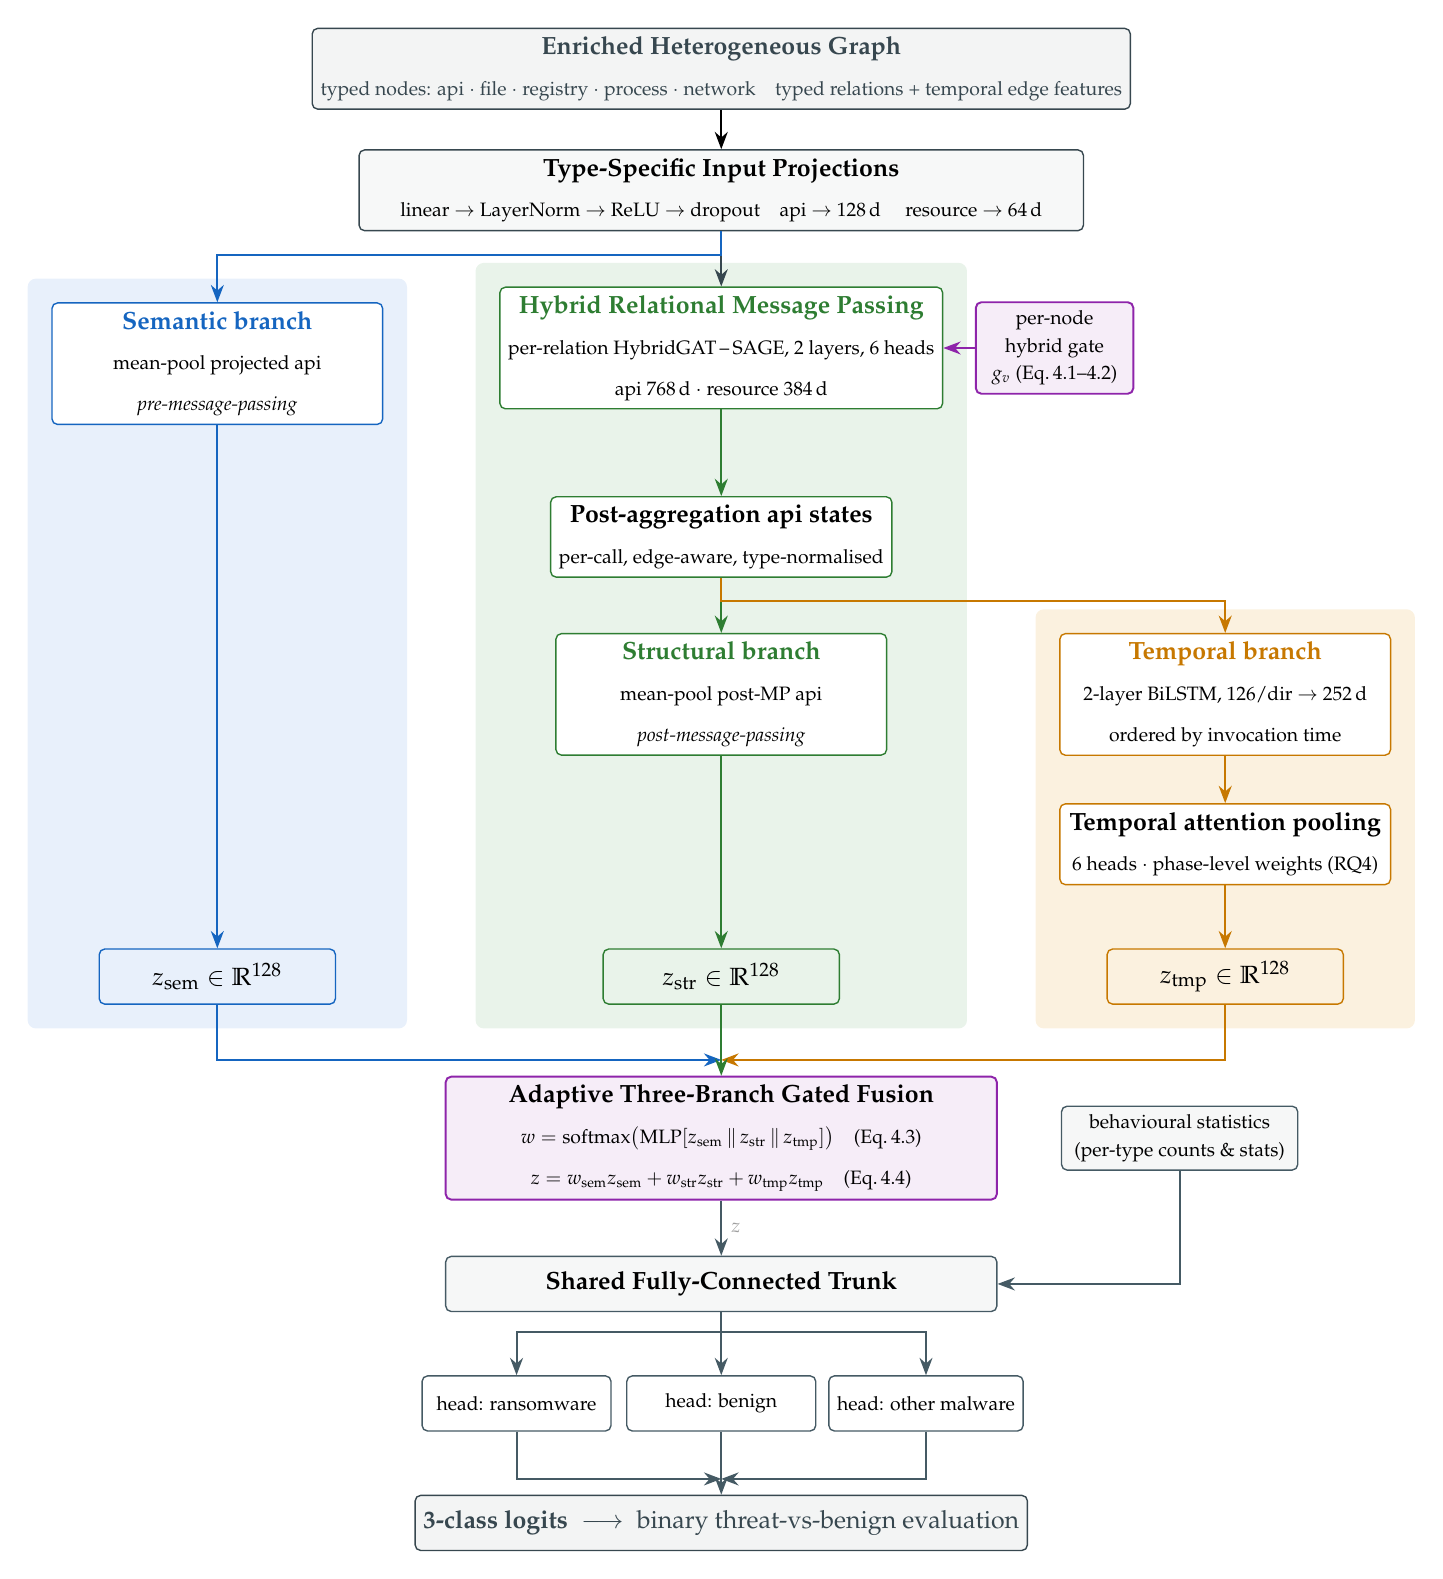
\begin{tikzpicture}[
    font=\small,
    >={Stealth[length=2.2mm]},
    block/.style={draw,rounded corners=2pt,align=center,inner sep=3pt,
                  minimum height=7mm,line width=0.5pt,fill=white},
    wide/.style={block,minimum width=92mm},
    branchbox/.style={block,minimum width=42mm},
    gate/.style={draw=cGate,fill=cGate!8,rounded corners=2pt,align=center,
                 inner sep=3pt,line width=0.7pt},
    flow/.style={->,line width=0.7pt},
    thinrel/.style={->,line width=0.5pt,gray!70},
    dim/.style={font=\scriptsize,gray!75},
  ]

  \node[wide,draw=cInput,fill=cInput!6,text=cInput] (graph)
    {\textbf{Enriched Heterogeneous Graph}\\[1pt]
     {\scriptsize typed nodes: api $\cdot$ file $\cdot$ registry $\cdot$ process $\cdot$ network\quad
      typed relations + temporal edge features}};

  \node[wide,below=5mm of graph,draw=cInput,fill=cInput!4] (proj)
    {\textbf{Type-Specific Input Projections}\\[1pt]
     {\scriptsize linear $\to$ LayerNorm $\to$ ReLU $\to$ dropout\quad
      api $\to$ 128\,d \quad resource $\to$ 64\,d}};
  \draw[flow] (graph) -- (proj);

  \def\xS{-64mm}\def\xR{0mm}\def\xT{64mm}

  \node[branchbox,draw=cSem,below=9mm of proj.south,xshift=\xS] (sempool)
    {\textbf{\textcolor{cSem}{Semantic branch}}\\[1pt]
     {\scriptsize mean-pool projected api}\\[1pt]{\scriptsize \emph{pre-message-passing}}};

  \node[branchbox,draw=cStr,below=7mm of proj.south,xshift=\xR] (mp)
    {\textbf{\textcolor{cStr}{Hybrid Relational Message Passing}}\\[1pt]
     {\scriptsize per-relation HybridGAT$\,$--$\,$SAGE, 2 layers, 6 heads}\\[1pt]
     {\scriptsize api 768\,d $\cdot$ resource 384\,d}};

  \node[branchbox,draw=cStr,below=11mm of mp] (states)
    {\textbf{Post-aggregation api states}\\[1pt]
     {\scriptsize per-call, edge-aware, type-normalised}};

  \node[branchbox,draw=cStr,below=7mm of states] (strpool)
    {\textbf{\textcolor{cStr}{Structural branch}}\\[1pt]
     {\scriptsize mean-pool post-MP api}\\[1pt]{\scriptsize \emph{post-message-passing}}};

  \node[branchbox,draw=cTmp,below=7mm of states.south,xshift=\xT] (lstm)
    {\textbf{\textcolor{cTmp}{Temporal branch}}\\[1pt]
     {\scriptsize 2-layer BiLSTM, 126/dir $\to$ 252\,d}\\[1pt]
     {\scriptsize ordered by invocation time}};

  \node[branchbox,draw=cTmp,below=6mm of lstm] (tpool)
    {\textbf{Temporal attention pooling}\\[1pt]
     {\scriptsize 6 heads $\cdot$ phase-level weights (RQ4)}};

  \node[block,draw=cTmp,fill=cBgTmp,below=8mm of tpool,minimum width=30mm] (ztmp)
    {$z_{\text{tmp}}\in\mathbb{R}^{128}$};
  \node[block,draw=cStr,fill=cBgStr,minimum width=30mm] (zstr) at (strpool |- ztmp)
    {$z_{\text{str}}\in\mathbb{R}^{128}$};
  \node[block,draw=cSem,fill=cBgSem,minimum width=30mm] (zsem) at (sempool |- ztmp)
    {$z_{\text{sem}}\in\mathbb{R}^{128}$};

  \draw[flow,cInput] (proj.south) -- ($(proj.south)+(0,-3mm)$) -| (mp.north);
  \draw[flow,cSem]  (proj.south) -- ($(proj.south)+(0,-3mm)$) -| (sempool.north);
  \draw[flow,cStr]  (mp) -- (states);
  \draw[flow,cStr]  (states) -- (strpool);
  \draw[flow,cTmp]  (states.south) -- ($(states.south)+(0,-3mm)$) -| (lstm.north);
  \draw[flow,cTmp]  (lstm) -- (tpool);
  \draw[flow,cSem] (sempool) -- (zsem);
  \draw[flow,cStr] (strpool) -- (zstr);
  \draw[flow,cTmp] (tpool) -- (ztmp);

  \node[gate,right=4mm of mp,minimum width=20mm,font=\scriptsize] (hgate)
    {per-node\\hybrid gate\\$g_v$ (Eq.\,4.1--4.2)};
  \draw[thinrel,cGate] (hgate) -- (mp);

  \node[gate,below=9mm of zstr,minimum width=70mm] (fuse)
    {\textbf{Adaptive Three-Branch Gated Fusion}\\[1pt]
     {\scriptsize $w=\mathrm{softmax}\big(\mathrm{MLP}[z_{\text{sem}}\,\|\,z_{\text{str}}\,\|\,z_{\text{tmp}}]\big)$\quad (Eq.\,4.3)}\\[1pt]
     {\scriptsize $z=w_{\text{sem}}z_{\text{sem}}+w_{\text{str}}z_{\text{str}}+w_{\text{tmp}}z_{\text{tmp}}$\quad (Eq.\,4.4)}};

  \draw[flow,cSem] (zsem.south) |- ($(fuse.north)+(0,2mm)$);
  \draw[flow,cTmp] (ztmp.south) |- ($(fuse.north)+(0,2mm)$);
  \draw[flow,cStr] (zstr) -- (fuse);

  \node[block,draw=cHead,fill=cHead!5,right=8mm of fuse,minimum width=30mm,font=\scriptsize] (behav)
    {behavioural statistics\\(per-type counts \& stats)};

  \node[block,draw=cHead,fill=cHead!5,below=7mm of fuse,minimum width=70mm] (trunk)
    {\textbf{Shared Fully-Connected Trunk}};
  \draw[flow,cHead] (fuse) -- (trunk) node[midway,right,dim]{$z$};
  \draw[flow,cHead] (behav.south) |- (trunk.east);

  \node[block,draw=cHead,below=8mm of trunk,xshift=-26mm,minimum width=24mm,font=\scriptsize] (hr){head: ransomware};
  \node[block,draw=cHead,below=8mm of trunk,xshift=0mm,minimum width=24mm,font=\scriptsize] (hb){head: benign};
  \node[block,draw=cHead,below=8mm of trunk,xshift=26mm,minimum width=24mm,font=\scriptsize] (hm){head: other malware};
  \draw[flow,cHead] (trunk.south) -- ++(0,-2.5mm) -| (hr.north);
  \draw[flow,cHead] (trunk.south) -- ++(0,-2.5mm) -| (hb.north);
  \draw[flow,cHead] (trunk.south) -- ++(0,-2.5mm) -| (hm.north);

  \node[block,draw=cInput,fill=cInput!6,below=8mm of hb,minimum width=70mm,text=cInput] (out)
    {\textbf{3-class logits} \;$\longrightarrow$\; binary threat-vs-benign evaluation};
  \draw[flow,cHead] (hr.south) |- ($(out.north)+(0,2mm)$);
  \draw[flow,cHead] (hb.south) -- (out.north);
  \draw[flow,cHead] (hm.south) |- ($(out.north)+(0,2mm)$);

  \begin{scope}[on background layer]
    \node[fill=cBgSem,rounded corners=3pt,fit=(sempool)(zsem),inner sep=3mm] {};
    \node[fill=cBgStr,rounded corners=3pt,fit=(mp)(states)(strpool)(zstr),inner sep=3mm] {};
    \node[fill=cBgTmp,rounded corners=3pt,fit=(lstm)(tpool)(ztmp),inner sep=3mm] {};
  \end{scope}
  \end{tikzpicture}}
  \caption[Architecture of the proposed HeteroTemporalGNN]{%
    Architecture of the proposed HeteroTemporalGNN. The enriched heterogeneous
    graph is projected per node type and split into three branches: the semantic
    branch reads the projected API representation \emph{before} message passing;
    the structural branch pools the API node states \emph{after} two layers of
    hybrid relational message passing; and the temporal branch applies a
    bidirectional LSTM with attention pooling over the same post-aggregation
    states ordered by invocation time. The three branch embeddings are integrated
    by an adaptive gated fusion mechanism, concatenated with behavioural
    statistics, and passed through a shared trunk to three single-logit heads,
    projected to a binary threat-versus-benign decision at evaluation.}
  \label{fig:architecture}
\end{figure}

\subsection{Type-Specific Input Projections}
\label{subsec:input_projections}

Node types carry features of very different dimensionality and
character (775-dimensional semantically enriched API vectors versus compact
numerical resource descriptors); each node type $\tau$ is therefore first
mapped into its own hidden space through a dedicated projection consisting of a
linear layer, layer normalisation, ReLU activation, and dropout. API nodes are
projected to a 128-dimensional hidden state and resource nodes to a
64-dimensional hidden state, reflecting their asymmetric informational roles.
The projected API representation, pooled per graph \emph{before} any
message passing or temporal mixing, is retained as the input to the semantic
branch of the fusion mechanism (Section~\ref{subsec:fusion}); it constitutes
the purest available summary of what the sample's operations mean,
uncontaminated by structural or temporal processing.

\subsection{Hybrid Relational Message Passing}
\label{subsec:hybrid_mp}

Structural reasoning is performed by two heterogeneous message-passing layers
following the type-aware formulation of Equation~\ref{eq:hetero_agg}: each
relation type maintains its own aggregation operator with independent
parameters, and per-type results are summed at each destination node.

The per-relation operator instantiates the hybrid design motivated in
Section~\ref{subsec:hybrid}, combining an edge-aware graph attention operator
(Section~\ref{subsec:gat}) with an edge-aware GraphSAGE operator
(Section~\ref{subsec:graphsage}). The decision to combine the two rather than
select one follows from their complementary failure modes in the behavioural
threat setting. Graph attention assigns learned importance weights to
neighbours, which is essential in behavioural graphs where discriminative
evidence is sparse: a single process-spawn or registry-persistence edge may
matter far more than thousands of routine file reads, and uniform aggregation
would dilute it. Attention coefficients additionally provide the
neighbour-level attribution signal required by RQ4. Attention scores are,
however, learned against the training distribution, and their reliability
degrades on neighbourhood patterns that differ from it, precisely the
condition produced by unseen threat families. GraphSAGE exhibits the inverse
profile: by learning a fixed, sampling-free aggregation function rather than
instance-specific weightings, it generalises robustly to nodes and topologies
never observed during training, the open-ended regime in which the set of
files, processes, and endpoints encountered at test time is unbounded, but it
treats all neighbours of a relation uniformly and therefore cannot emphasise
the rare, salient interaction. Neither inductive bias is adequate alone for a
detector that must simultaneously discriminate sparse evidence on known
behaviour and remain stable on novel behaviour; the hybrid operator retains
both and learns, per node and per feature, which to trust.

Both operators consume the temporal edge features of
Section~\ref{subsec:temporal_features} on relations that carry them, but they
ingest those features differently, which is part of what makes them
complementary. In the attention operator, the projected edge features enter the
unnormalised attention score of Equation~\ref{eq:gat_score} as a third additive
term alongside the source and target contributions, so that edge context
directly modulates how strongly each neighbour is weighted. The GraphSAGE
operator, by contrast, is a modified, edge-aware variant of the standard
formulation in Equation~\ref{eq:graphsage}: rather than aggregating raw
neighbour states, each neighbour message is first formed as
$\mathbf{m}_{uv} = \mathbf{h}_u + \mathbf{W}_e\,\mathbf{e}_{uv}$, additively
injecting the projected edge features before the mean aggregation, so the
inductive pathway preserves the temporal edge signal without introducing any
per-pair weighting. The two operator outputs are then reconciled through a
learned, feature-wise gate. Given the
attention output $\mathbf{h}^{\mathrm{GAT}}_v$ and the inductive output
$\mathbf{h}^{\mathrm{SAGE}}_v$ for node $v$, the gate is computed as
\begin{equation}
  \mathbf{g}_v = \sigma\!\Bigl(
    \mathrm{MLP}\!\bigl[\,
      \mathbf{h}^{\mathrm{GAT}}_v \,\|\,
      \mathbf{h}^{\mathrm{SAGE}}_v \,\|\,
      \lambda_d \bigl|\mathbf{h}^{\mathrm{GAT}}_v - \mathbf{h}^{\mathrm{SAGE}}_v\bigr|
    \,\bigr]\Bigr),
  \label{eq:hybrid_gate}
\end{equation}
where $\sigma$ is the elementwise sigmoid, $\lambda_d = 2.0$ scales the
disagreement term, and the gate MLP contains a single hidden layer with
dropout. The fused representation is the convex combination
\begin{equation}
  \mathbf{h}_v = \mathbf{g}_v \odot \mathbf{h}^{\mathrm{GAT}}_v
  + (\mathbf{1} - \mathbf{g}_v) \odot \mathbf{h}^{\mathrm{SAGE}}_v.
  \label{eq:hybrid_fuse}
\end{equation}
Including the absolute disagreement
$|\mathbf{h}^{\mathrm{GAT}}_v - \mathbf{h}^{\mathrm{SAGE}}_v|$ in the gate
input allows the gate to detect precisely those nodes on which the two
inductive biases diverge and to arbitrate between them; where the operators
agree, the choice is immaterial and the gate can remain neutral. The final
bias of the gate MLP is initialised to $-0.85$, so that
$\sigma(-0.85) \approx 0.30$ and the model initially weights the inductive
operator at roughly 70\%. This $70/30$ split is only a starting point, not a
fixed ratio: because the gate $\mathbf{g}_v$ of Equation~\ref{eq:hybrid_gate}
is computed per node and per feature from the operator outputs themselves, the
actual mixture is decided automatically at each node, and may favour either
operator once training is under way. The initialisation merely prevents the
attention pathway, whose scores are unreliable at the start of training, from
dominating early optimisation, while leaving the network free to shift weight
toward attention as its coefficients become informative. A small regularisation term
($10^{-3}$) discourages premature gate collapse, and per-relation gate
statistics are monitored throughout training.

Each layer uses 6 attention heads with concatenated head outputs, so that API
nodes reach a post-aggregation width of $128 \times 6 = 768$ and resource
nodes $64 \times 6 = 384$; layer normalisation is applied per type after each
layer, a residual connection is added wherever a layer's input and output
widths coincide, easing gradient flow through the stack, and the result then
passes through a ReLU nonlinearity and dropout. After the second
layer, the API node states, mean-pooled per graph,
form the input to the structural branch of the fusion mechanism: a summary of
the sample's relational topology as refined by hybrid message passing.

\subsection{Temporal Sequence Modelling}
\label{subsec:temporal_branch}

The temporal branch operates on the post-aggregation API node states, ordered
by their invocation timestamps within each graph, and therefore observes
sequences whose elements already encode semantic and relational context. The
ordered sequence is processed by a two-layer bidirectional LSTM
(Section~\ref{subsec:bilstm}) with 126 hidden units per direction, yielding a
252-dimensional output per API call that is contextualised by both the
preceding and the following execution history as in
Equation~\ref{eq:bilstm}. Bidirectionality is appropriate here because
classification is performed over fully observed traces, so future context is
legitimately available; an event such as a registry modification acquires a
different significance when followed by mass file writes than when followed by
process termination.

The per-call outputs are condensed into a graph-level temporal embedding by a
multi-head temporal attention pooling layer with 6 heads, which learns to
weight the calls by their discriminative relevance rather than averaging
uniformly over sequences in which malicious activity may occupy only a small
fraction of the trace. The attention weights produced by this layer are
retained for the attribution analysis of RQ4, since they identify \emph{which
phases} of execution drove a prediction. The pooled temporal embedding is
projected to the common fusion dimension and forms the temporal branch input.

The BiLSTM is the temporal backbone used throughout this work, chosen for its
maturity and stable optimisation. The slot it occupies is, however, deliberately
modular: any sequence model exposing the same per-call interface, such as the
selective state-space (Mamba) model of Section~\ref{sec:mamba}, can be
substituted without altering the rest of the architecture. This keeps the design
open to experimentation with lower-complexity alternatives on long execution
traces, while fixing the BiLSTM as the configuration evaluated in this thesis.

\subsection{Adaptive Three-Branch Gated Fusion}
\label{subsec:fusion}

The three branches yield three graph-level embeddings in a common
128-di\-men\-sional space: the semantic embedding
$\mathbf{z}^{\mathrm{sem}}$ (pooled pre-aggregation API representations,
Section~\ref{subsec:input_projections}), the structural embedding
$\mathbf{z}^{\mathrm{str}}$ (pooled post-aggregation API states,
Section~\ref{subsec:hybrid_mp}), and the temporal embedding
$\mathbf{z}^{\mathrm{tmp}}$ (attention-pooled BiLSTM output,
Section~\ref{subsec:temporal_branch}). Rather than concatenating these
embeddings with fixed importance, the framework integrates them through an
adaptive gated fusion mechanism that computes per-sample branch weights,
\begin{equation}
  \mathbf{w} = \mathrm{softmax}\!\Bigl(
    \mathrm{MLP}\!\bigl[\,
      \mathbf{z}^{\mathrm{sem}} \,\|\,
      \mathbf{z}^{\mathrm{str}} \,\|\,
      \mathbf{z}^{\mathrm{tmp}}
    \,\bigr]\Bigr) \in \mathbb{R}^{3},
  \label{eq:branch_gate}
\end{equation}
where the gate MLP consists of a 128-unit hidden layer with layer
normalisation, GELU activation, and dropout. The fused graph embedding is the
weighted combination
\begin{equation}
  \mathbf{z} = w_{\mathrm{sem}}\,\mathbf{z}^{\mathrm{sem}}
             + w_{\mathrm{str}}\,\mathbf{z}^{\mathrm{str}}
             + w_{\mathrm{tmp}}\,\mathbf{z}^{\mathrm{tmp}}.
  \label{eq:branch_fusion}
\end{equation}

This mechanism realises Objective~4 of Section~\ref{sec:objectives} and serves
two distinct purposes. As a modelling device, it acknowledges that the
relative informativeness of the three dimensions varies across samples: a
threat detected primarily through its API substitution pattern is a
semantically driven decision, whereas one detected through its encryption
burst is temporally driven, and a fixed combination would be suboptimal for
both. As an interpretability device, the per-sample weight vector $\mathbf{w}$
constitutes a direct, quantitative attribution of each prediction to the three
behavioural dimensions, providing the dimension-level explanation signal
required by RQ4 without any post-hoc approximation.

Two safeguards prevent degenerate gate behaviour. During training, each branch
embedding is independently zeroed with probability $0.05$ (branch dropout),
which forces the classifier to remain functional when any single branch is
absent and prevents over-reliance on one dimension. In addition, a soft
entropy-based balance penalty,
\begin{equation}
  \mathcal{L}_{\mathrm{bal}}
  = \lambda_{b}\;
    \mathbb{E}\!\left[
      \max\!\Bigl( 0,\; H^{*} - \tfrac{H(\mathbf{w})}{\log 3} \Bigr)
    \right],
  \qquad
  H(\mathbf{w}) = -\sum_{i} w_i \log w_i,
  \label{eq:branch_balance}
\end{equation}
with target entropy $H^{*} = 0.75$ and $\lambda_b = 0.01$, penalises the gate
only when its normalised entropy collapses below the target. The penalty
deliberately does \emph{not} force equal branch usage: it permits arbitrary
specialisation per sample while preventing the gate from collapsing globally
onto a single branch early in training, before the slower-converging branches
have become informative.

\subsection{Behavioural Statistics and Classification Head}
\label{subsec:classifier}

The fused embedding is concatenated with a compact vector of per-type
behavioural statistics, comprising three values per node type (a normalised
node count and two aggregate feature statistics) computed per graph, which
supplies coarse contextual information (such as the overall scale of file and
registry activity) that the mean-based pooling operations, being invariant to
node count, cannot recover from the branch embeddings alone. The combined vector passes through a
shared fully connected trunk followed by three parallel single-logit heads,
one per class (ransomware, benign, other malware), whose outputs are
concatenated into the final logit vector. Separating the heads over a shared
trunk allows each class boundary to be refined independently while the trunk
representation remains common, which is advantageous under the class imbalance
described next.

\section{Training Procedure}
\label{sec:training}

This section specifies how the model is trained, covering the loss formulation
and sampling strategy, the regularisation applied for robustness, and the
optimisation protocol.

\subsection{Class Imbalance Handling}
\label{subsec:imbalance}

Ransomware is the rarest class by more than an order of magnitude
(Section~\ref{subsec:preprocessing}), and standard cross-entropy training
therefore collapses toward the majority classes. Two complementary
countermeasures are applied.

First, the task loss is the focal loss of Lin et al.~\cite{lin2017focal},
\begin{equation}
  \mathcal{L}_{\mathrm{focal}}
  = -\,\alpha_{y}\,\bigl(1 - p_{y}\bigr)^{\gamma}\,\log p_{y},
  \label{eq:focal}
\end{equation}
where $p_{y}$ is the predicted probability of the true class $y$,
$\gamma = 2$ is the focusing parameter, and
$\boldsymbol{\alpha} = (0.39, 0.39, 0.42)$ are per-class weighting
coefficients for ransomware, benign, and other malware respectively. The
modulating factor $(1-p_y)^{\gamma}$ down-weights well-classified examples and
concentrates gradient signal on hard ones, which under imbalance are
predominantly minority-class samples.

Second, weighted oversampling is applied at the data-loader level, drawing
training samples with class-dependent replacement weights of $9.0$ for
ransomware, $3.5$ for benign, and $1.2$ for other malware. Oversampling
increases the frequency with which minority-class gradients are observed,
while the focal loss shapes the per-sample gradient magnitude, so the two
mechanisms address the imbalance at complementary points of the optimisation.
This division of labour explains why the focal weights are nearly uniform rather
than skewed toward ransomware. The oversampler already concentrates on the rare
classes, drawing ransomware several times more often than other malware, so the
focal $\alpha$ coefficients do not also need to privilege ransomware; favouring
the same class through both mechanisms at once would over-correct and
destabilise training. The $\alpha$ values are therefore left close to balanced,
and the slightly higher coefficient on the other-malware class ($0.42$ against
$0.39$ for ransomware and benign) instead compensates for that class being the
\emph{least} oversampled, keeping the net per-class emphasis even once the two
mechanisms combine.

The total training objective combines the task loss with the branch balance
penalty of Equation~\ref{eq:branch_balance} and the hybrid gate
regularisation of Section~\ref{subsec:hybrid_mp}:
\begin{equation}
  \mathcal{L}
  = \mathcal{L}_{\mathrm{focal}}
  + \mathcal{L}_{\mathrm{bal}}
  + \mathcal{L}_{\mathrm{gate}}.
  \label{eq:total_loss}
\end{equation}

\subsection{Regularisation and Robustness}
\label{subsec:regularisation}

The model is further regularised, beyond the gate-level safeguards already
described, with dropout of $0.3$ in the projection and aggregation layers and
$0.2$ within the LSTM, weight decay of $10^{-3}$, and gradient-norm clipping at
$1.0$. In addition, semantic perturbation training is applied: with
probability $0.2$ per training batch, zero-mean Gaussian noise with standard
deviation $0.05$ is added to the temporal edge features. Because both
aggregation operators of Section~\ref{subsec:hybrid_mp} consume these
features, the perturbation discourages brittle dependence on exact timing
values and simulates the measurement noise inherent in sandbox timestamping.
Perturbation is applied strictly during training and never during validation
or testing.

\subsection{Optimisation Protocol}
\label{subsec:optimisation}

The model is trained with the AdamW optimiser~\cite{loshchilov2019adamw} at a
base learning rate of $10^{-4}$ and weight decay of $10^{-3}$, with gradients
clipped to a maximum norm of $1.0$ for stability. The learning rate is reduced
on plateau of the validation metric. Training proceeds for up to 125
epochs with early stopping after 20 epochs without improvement in validation
macro-F1, which is also the checkpoint-selection criterion; macro-F1 weights
all three classes equally and is therefore the appropriate model-selection
signal under imbalance. Because graph sizes span four orders of magnitude,
batches are formed by a bucketed size-aware sampler that groups graphs of
comparable API node count and assigns larger batch sizes to buckets of smaller
graphs (from 64 graphs per batch below 10{,}000 API nodes down to single-graph
batches above 100{,}000), keeping per-batch memory approximately constant
without discarding any portion of the size distribution.

\section{Evaluation}
\label{sec:evaluation}

This section specifies how the trained model is assessed. It defines the
threat-versus-benign evaluation framing, the metrics used, the protocols for
measuring generalisation to unseen threat families and robustness to
behavioural perturbation, the baseline families against which the framework is
compared, and the ablation design that isolates each component's contribution.

\subsection{Three-Class Training with Binary Threat Evaluation}
\label{subsec:binary_projection}

The framework is trained over three internal classes but evaluated primarily
as a binary threat detector. This is a deliberate design decision rather than
an inconsistency, and its rationale is twofold, spanning a learning perspective
and an operational one.

From a learning perspective, the three-class classification was intentionally
designed as a more challenging and behaviour-aware learning task. Although
ransomware is a subtype of malware, it exhibits distinct behavioural
characteristics and attack objectives, including a characteristic temporal
signature (encryption bursts, rapid mass file modification) that would be
diluted if merged into an undifferentiated threat class. By separating benign,
malware, and ransomware samples during training, the model is encouraged to
learn fine-grained, deep behavioural patterns instead of only a broad
malicious-versus-benign boundary, and the dedicated ransomware class forces the
temporal branch to learn its signature explicitly. The same holds for general
malware, whose distinguishing structural relationships among processes, files,
registry, and network activity the structural branch is likewise compelled to
represent, and which would be flattened were all threats collapsed into a
single class. This is particularly
important for zero-day detection, where previously unseen threats may not share
exact characteristics with known samples: assessing a novel sample on these
deep behavioural patterns allows it to be pushed to the threat side rather than
misclassified as benign. A direct binary formulation does not compel the model
to learn these underlying behaviours as deeply, leaving a previously unseen
threat more likely to be assigned to the benign class. Consequently, the binary
threat-detection task benefits from the model's prior exposure to three
distinct behavioural patterns.

From an operational perspective, the question a deployed detector must answer
is binary: is the sample a threat or not. The evaluation therefore projects
the three-class output onto the binary decision
\begin{equation}
\hat{y}_{\mathrm{bin}} =
\begin{cases}
\text{threat}, & \hat{y} \in \{\text{ransomware},\ \text{other malware}\},\\[2pt]
\text{benign}, & \hat{y} = \text{benign},
\end{cases}
\label{eq:binary_projection}
\end{equation}
and all headline detection results are reported under this projection, with
the three-class metrics reported alongside for completeness. Under the binary
projection, the operationally critical error is a missed threat (a malicious
sample classified as benign); confusion \emph{between} the two malicious
classes is irrelevant to detection performance.

\subsection{Evaluation Metrics}
\label{subsec:metrics}

Performance is measured with accuracy, per-class and macro-averaged
precision, recall, and F1-score, the area under the precision--recall curve
(AUPRC), and the false positive rate (FPR). Macro-averaged metrics and AUPRC
are preferred over accuracy and ROC-based measures because both remain
informative under heavy class imbalance, where accuracy saturates and ROC
curves present an optimistic picture. Under the binary projection, threat
recall and the absolute count of missed threats are reported explicitly,
since a single missed ransomware sample carries disproportionate operational
cost; the FPR on benign software quantifies the complementary operational
burden of false alarms. Following the operational considerations of
Section~\ref{subsec:early_stage} and Cen et al.~\cite{cen2021ransomware},
time-to-detect is additionally assessed by evaluating predictions over
truncated prefixes of the execution trace, measuring how early in execution a
threat verdict becomes available.

\subsection{Generalisation Protocol: Leave-Family-Out Evaluation}
\label{subsec:lofo}

Random splits over-estimate real-world performance because samples of the same
threat family appear on both sides of the split, allowing a model to succeed
by memorising family-specific artefacts. To measure generalisation to genuinely
novel threats (RQ5), a leave-family-out protocol is employed: a set of threat
families is withheld entirely from training and validation, and an evaluation
corpus is assembled containing all samples of the withheld families alongside
200 benign samples and 55 samples of known (training-time) malware families
drawn from the held-out splits, together with all available ransomware
samples. Disjointness between the withheld families and all training material
is programmatically enforced, and the evaluation manifest is persisted so the
exact corpus composition is reproducible. Under this protocol, correct
detection of the withheld families cannot be attributed to memorisation; it
requires the learned semantic, structural, and temporal abstractions to
transfer, which is precisely the capability the framework is designed to
provide.

\subsection{Robustness to Behavioural Perturbation}
\label{subsec:robustness_eval}

Generalisation to unseen families addresses only one half of RQ5; the other is
robustness to deliberate perturbation of the behavioural trace itself. A
complementary protocol therefore subjects the trained model, without any
retraining, to a battery of adversarial transformations applied to the
evaluation graphs at inference time, and measures the resulting change in threat
recall relative to the clean corpus. Distinct from the semantic perturbation
applied during training (Section~\ref{subsec:regularisation}), which hardens the
model, these transformations are introduced purely at evaluation time as a
stress test. The same transformed graphs are presented to the classical and
static baselines of Section~\ref{subsec:baselines}, so that the degradation of
each detection paradigm can be compared directly on identical inputs.

The perturbations are organised into tracks, each targeting the inductive bias
of a different paradigm while preserving the malicious intent of the trace:

\begin{description}[leftmargin=0pt, labelwidth=0pt, labelsep=\parskip, style=nextline]

\item[\textbf{Lexical substitution.}] A fraction of API names is renamed to
semantically equivalent aliases or out-of-vocabulary variants, the most
frequent core operations are preserved, and the trace is optionally diluted with
benign-looking calls. This track targets models that depend on token identity or
frequency, such as unigram feature counts.

\item[\textbf{Ordering perturbation.}] Benign calls are interleaved into the
sequence and local call order is shuffled, leaving the multiset of operations
largely intact. This track targets models that depend on adjacent-order
statistics, such as bigram feature counts.

\item[\textbf{Combined perturbation.}] The lexical and ordering tracks are
applied together, representing a stronger adversary that degrades both identity
and order simultaneously.

\item[\textbf{Semantic-vector substitution.}] Operating directly on the semantic
representation, a fraction of API embeddings is replaced with that of their
nearest functional neighbour, with replacement by unrelated random vectors
serving as a control. This track isolates whether detection depends on the exact
identity of an operation or on its functional meaning.

\end{description}

Because each transformation alters the surface form of a trace while leaving its
malicious behaviour intact, a model that encodes behavioural meaning rather than
surface artefacts should degrade only marginally, whereas a counting- or
order-based model should degrade sharply. This protocol therefore
operationalises the semantic-robustness claim of RQ1 and the
perturbation-robustness requirement of RQ5. The concrete perturbation parameters
and the per-model degradation they induce are reported in
Chapter~\ref{chap:results}.

\subsection{Baseline Families}
\label{subsec:baselines}

The framework is compared against one representative from each major
methodological family identified in Table~\ref{tab:literature_comparison}, each
trained and evaluated on identical splits:

\begin{description}[leftmargin=0pt, labelwidth=0pt, labelsep=\parskip, style=nextline]

\item[\textbf{Classical machine learning.}] Random Forest and gradient-boosted
tree (XGBoost) classifiers over TF-IDF unigram and bigram representations of
the API call sequence, representing the static
feature-engineering paradigm of Section~\ref{subsec:static_ml}.

\item[\textbf{Sequential deep learning.}] A recurrent sequence classifier over
the ordered API call sequence, representing the sequence-only paradigm of
Section~\ref{subsec:sequential_dl}, which preserves ordering but discards
relational structure.

\item[\textbf{Static graph neural networks.}] Heterogeneous GCN and GAT
models trained on the same graphs under a strict protocol in which semantic
API embeddings, temporal edges and timestamps, and behavioural statistics are
all withheld, isolating the contribution of static relational structure alone.

\item[\textbf{LLM-based behavioural analysis.}] An LLM-driven classifier in
the style of BEACON~\cite{perera2023beacon}, in which execution traces are
rendered as natural-language behavioural descriptions and classified by a
large language model, representing the semantic-only paradigm of
Section~\ref{subsec:semantic_llm}.

\end{description}

This selection ensures that each behavioural dimension is represented in
isolation by at least one baseline, so that the comparison directly tests the
central claim of RQ3: that joint modelling outperforms each single-paradigm
alternative.

\subsection{Ablation Design}
\label{subsec:ablations}

The contribution of each architectural component is quantified by ablating the
single trained model under otherwise identical conditions: one component is
removed or perturbed at evaluation time and the resulting change in detection
performance is measured. The ablation set comprises:
\begin{enumerate}[leftmargin=*]
  \item \emph{Drop-one branch removal.} Each fusion branch is removed in turn
        (semantic, structural, temporal) by zeroing it through the
        branch-dropout pathway, measuring the \emph{marginal} contribution of
        each dimension in the presence of the others.
  \item \emph{Keep-one branch isolation.} A single branch is retained with the
        other two suppressed (se\-mantic-only, struc\-tural-only,
        tem\-poral-only), together with the se\-mantic--temporal pairing that
        withholds graph
        structure, measuring the \emph{standalone} contribution of each
        dimension and the \emph{joint} contribution of a pair.
  \item \emph{Aggregator substitution.} The hybrid aggregator of
        Equation~\ref{eq:hybrid_fuse} is replaced by its pure attention and
        pure inductive constituents.
  \item \emph{Temporal-feature removal.} The engineered temporal edge features
        are withheld.
  \item \emph{Semantic substitution.} The pretrained semantic embeddings are
        replaced with uninformative vectors, isolating the contribution of
        learned semantics over symbolic identity.
\end{enumerate}
Together, the drop-one and keep-one ablations quantify the individual and joint
contribution of the semantic, structural, and temporal dimensions and so
address RQ2 directly; the temporal-feature and semantic substitutions isolate
the semantic-generalisation question of RQ1; and the aggregator substitution
attributes performance to the architectural composition itself. All of these
are component sensitivity analyses of the single trained model rather than
separately retrained single-branch networks; they therefore quantify the
model's \emph{reliance} on each component at inference time rather than the
standalone capability of a component trained in isolation, and are reported and
interpreted strictly on those terms. In addition, the
per-sample fusion weights of Equation~\ref{eq:branch_gate}, the hybrid gate
statistics, and the temporal attention distributions are analysed qualitatively
on correctly and incorrectly classified samples to provide the attribution
evidence required by RQ4. The measured effect of each ablation is reported in
Chapter~\ref{chap:results}.

\section{Hardware and Software Configuration}
\label{sec:hw_sw_config}

Training and evaluation are carried out on a single high-memory GPU. The
dominant resource constraint is GPU memory rather than compute: the largest
behavioural graphs span on the order of $10^5$ API nodes, and each API node
carries a 768-dimensional semantic embedding, so the densest graphs must be
processed as single-graph batches (Section~\ref{subsec:optimisation}). A device
with at least 80\,GB of VRAM is therefore required to process the full size
distribution without out-of-memory failures, and lower-memory devices can train
the model only by truncating or down-sampling the largest graphs, which would
compromise the size-preserving design. The implementation is built in Python on
the PyTorch~\cite{paszke2019pytorch} deep-learning framework, with heterogeneous
graph construction and typed message passing provided by PyTorch
Geometric~\cite{fey2019pyg}; the semantic embeddings of
Section~\ref{subsec:semantic_enrichment} are produced through the
\texttt{sentence-transformers} stack. The complete configuration is summarised
in Table~\ref{tab:hw_sw_config}.

\begin{table}[htbp]
\centering
\caption{Hardware and software configuration used for training and evaluation.}
\label{tab:hw_sw_config}
\begin{tabular}{ll}
\toprule
\textbf{Component} & \textbf{Specification} \\
\midrule
\multicolumn{2}{l}{\textit{Hardware}} \\
GPU (reported)        & NVIDIA RTX~PRO~6000 workstation, 96\,GB VRAM \\
Minimum VRAM          & 80\,GB (avoids out-of-memory on the largest graphs) \\
Equivalent devices    & NVIDIA A100 or H100, 80\,GB \\
\midrule
\multicolumn{2}{l}{\textit{Software}} \\
Language              & Python \\
Deep learning         & PyTorch~$\geq$2.1, PyTorch Geometric~$\geq$2.5 \\
Semantic enrichment   & sentence-transformers, transformers, tokenizers (MPNet) \\
Numerical / data      & NumPy, SciPy, pandas \\
Metrics / plotting     & scikit-learn, Matplotlib, seaborn \\
Optional (Mamba)      & mamba-ssm, causal-conv1d (CUDA-only) \\
\bottomrule
\end{tabular}
\end{table}

The Mamba temporal backbone (Section~\ref{subsec:temporal_branch}) is optional:
its \texttt{mamba-ssm} and \texttt{causal-conv1d} dependencies compile custom
CUDA kernels and are installed only on the training host, whereas the default
bidirectional LSTM backbone has no such dependency and remains operable on any
supported device.

\section{Chapter Summary}
\label{sec:methodology_summary}

This chapter specified the complete experimental methodology: a behavioural
corpus of malicious and benign execution traces transformed into schema-aware
heterogeneous graphs with five typed node classes and five typed relations; semantic
enrichment of API nodes through MPNet-based sentence embeddings; engineered
temporal edge features capturing pacing, acceleration, and burst behaviour;
and the proposed HeteroTemporalGNN architecture, which combines hybrid
GAT--SAGE relational aggregation, bidirectional LSTM temporal modelling with
attention pooling, and an adaptive three-branch gated fusion mechanism whose
weights double as dimension-level attribution signals. Training employs focal
loss and weighted oversampling against severe class imbalance, with branch
balance regularisation, semantic perturbation, and a size-aware batching
scheme. Evaluation combines a binary threat-versus-benign projection of the
three-class output with imbalance-robust metrics, a leave-family-out protocol
for cross-family generalisation, four baseline families covering each
single-paradigm alternative, and a systematic ablation design.
Chapter~\ref{chap:results} reports the experimental results, covering the
component-attribution and ablation studies, the comparison against the four
baseline families, and the generalisation and robustness evaluations defined
above.

\chapter{Experiments and Results}
\label{chap:results}

This chapter presents the experiments conducted with the framework of
Chapter~\ref{chap:methodology} and the results they yield, following the
evaluation methodology of Section~\ref{sec:evaluation}. It reports the
component-attribution and ablation studies that isolate the contribution of
each branch and mechanism, the comparison against the four baseline families,
and the evaluations of cross-family generalisation and robustness to
behavioural perturbation.

% Content to be completed.

\chapter{Limitations and Future Work}
\label{chap:future_work}

This chapter discusses the limitations of the present work and the directions
in which the framework could be extended.

% Content to be completed.

% ============================================================
% BIBLIOGRAPHY
% ============================================================
\bibliographystyle{IEEEtran}
\bibliography{bibThesis}

\end{document}